\chapter{Alternative Studies, 2017 Analysis}
\label{sec:data_alt_studies}
The largest concern for the analysis presented was the poor posterior predictive p-value, driven primarily by the modelling of the FGD1 CCOther selection. A number of compatibility studies were made to study the effects of this and various other model choices, e.g. using BeRPA and 2p2h shape.

For the alternative studies that had the largest effect on the ND280 fit, we propagate the parameter values results to SK and inspect  the difference relative the reference model using the full data set. For the oscillation parameters we fix them to those in \autoref{tab:osc_pars} and the SK detector parameters are set to their prior central values and are not varied.

The procedure mimics that of the posterior predictive method, in which MCMC steps are randomly selected after burn-in to give a parameter set $\vec{x}$, used to reweight the Monte-Carlo prediction which is filled in a two-dimensional histogram ($N_{toys}$ vs $E_{rec}$ here). A Gaussian is then fit to the bin-by-bin distributions and the mean and rms is extracted and taken as the central value and 1$\sigma$.

\section{Neutrino vs Anti-Neutrino}
The data-sets used for the full fit (runs 2 to 6) spanned neutrino (runs 2 to 4) and anti-neutrino runs (runs 5 to 6), as shown in  \autoref{tab:pot_2017}. As seen in the table, the FHC/RHC ratio is roughly 1.5 and looking at \autoref{tab:event_rates_2017} the FHC/RHC event rate ratio is 3.4. Hence the full run 2 to 6 fit is dominated by FHC running and hence by neutrino rather than anti-neutrino interactions.

To investigate the compatibility between neutrino and anti-neutrino data at T2K, we perform data fits to run 2 to 4 data and to run 5 to 6 data separately, comparing results to the full fit. Due to the different event rates we expect larger constraints on parameters from the FHC data (run 2 to 4) than the RHC data (run 5 to 6), and the overall constraint from the full fit to come primarily from the FHC data. 

\autoref{fig:flux_data_nd280_nuvsnubar} shows the ND280 flux parameters after the fit with the prefit uncertainty band in red. As expected, the anti-neutrino fit barely moves the central values for the FHC parameters, and the small movements are due to the covariance matrix penalty tying the FHC and RHC flux together. The full fit often settles between the two separate fits' central values, but in cases of extreme pulls the full fit sits closer to the neutrino fit. The neutrino-only fit pulls the extreme cases a little further (e.g. e.g. FHC \numu $\sim1\text{ GeV}$, high $E_\nu$ \numu and \numubar), highlighting the slight tension with the prior covariance matrix. Generally the flux parameters are compatible throughout and often well within $1\sigma$ of each other.
\begin{figure}[h]
	\begin{subfigure}[t]{0.10\textwidth}
		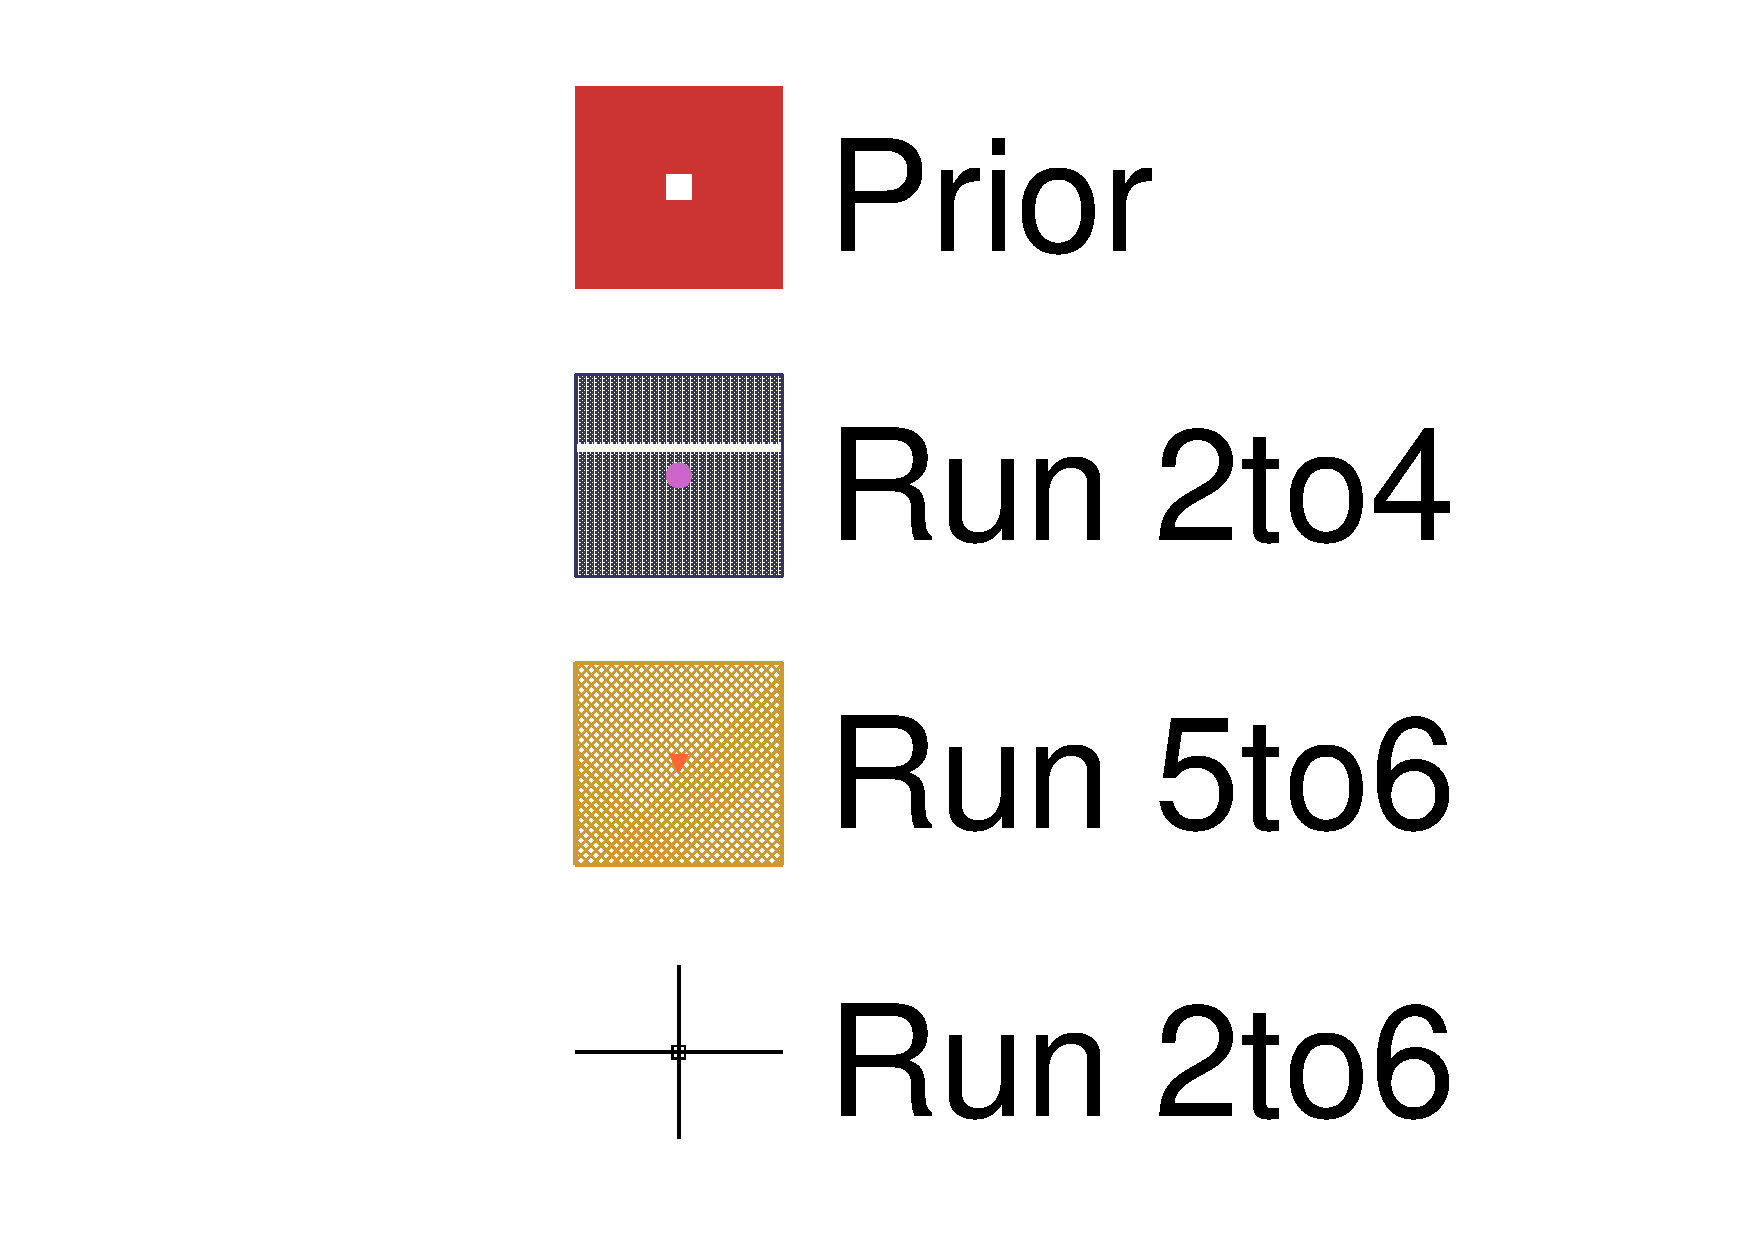
\includegraphics[width=\textwidth, trim={0mm 0mm 0mm 0mm}, clip,page=1]{figures/mach3/data/alt/2017b_Run2to4_Data_merge_2017b_Run56_Data_merge_2017b_NewData_NewDet_UpdXsecStep_2Xsec_4Det_5Flux_0}
	\end{subfigure}
	
	\begin{subfigure}[t]{0.24\textwidth}
		\includegraphics[width=\textwidth, trim={0mm 0mm 0mm 0mm}, clip,page=2]{figures/mach3/data/alt/2017b_Run2to4_Data_merge_2017b_Run56_Data_merge_2017b_NewData_NewDet_UpdXsecStep_2Xsec_4Det_5Flux_0}
	\end{subfigure}
	\begin{subfigure}[t]{0.24\textwidth}
		\includegraphics[width=\textwidth, trim={0mm 0mm 0mm 0mm}, clip,page=3]{figures/mach3/data/alt/2017b_Run2to4_Data_merge_2017b_Run56_Data_merge_2017b_NewData_NewDet_UpdXsecStep_2Xsec_4Det_5Flux_0}
	\end{subfigure}
	\begin{subfigure}[t]{0.24\textwidth}
		\includegraphics[width=\textwidth, trim={0mm 0mm 0mm 0mm}, clip,page=4]{figures/mach3/data/alt/2017b_Run2to4_Data_merge_2017b_Run56_Data_merge_2017b_NewData_NewDet_UpdXsecStep_2Xsec_4Det_5Flux_0}
	\end{subfigure}
	\begin{subfigure}[t]{0.24\textwidth}
		\includegraphics[width=\textwidth, trim={0mm 0mm 0mm 0mm}, clip,page=5]{figures/mach3/data/alt/2017b_Run2to4_Data_merge_2017b_Run56_Data_merge_2017b_NewData_NewDet_UpdXsecStep_2Xsec_4Det_5Flux_0}
	\end{subfigure}
	
	\begin{subfigure}[t]{0.24\textwidth}
		\includegraphics[width=\textwidth, trim={0mm 0mm 0mm 0mm}, clip,page=6]{figures/mach3/data/alt/2017b_Run2to4_Data_merge_2017b_Run56_Data_merge_2017b_NewData_NewDet_UpdXsecStep_2Xsec_4Det_5Flux_0}
	\end{subfigure}
	\begin{subfigure}[t]{0.24\textwidth}
		\includegraphics[width=\textwidth, trim={0mm 0mm 0mm 0mm}, clip,page=7]{figures/mach3/data/alt/2017b_Run2to4_Data_merge_2017b_Run56_Data_merge_2017b_NewData_NewDet_UpdXsecStep_2Xsec_4Det_5Flux_0}
	\end{subfigure}
	\begin{subfigure}[t]{0.24\textwidth}
		\includegraphics[width=\textwidth, trim={0mm 0mm 0mm 0mm}, clip,page=8]{figures/mach3/data/alt/2017b_Run2to4_Data_merge_2017b_Run56_Data_merge_2017b_NewData_NewDet_UpdXsecStep_2Xsec_4Det_5Flux_0}
	\end{subfigure}
	\begin{subfigure}[t]{0.24\textwidth}
		\includegraphics[width=\textwidth, trim={0mm 0mm 0mm 0mm}, clip,page=9]{figures/mach3/data/alt/2017b_Run2to4_Data_merge_2017b_Run56_Data_merge_2017b_NewData_NewDet_UpdXsecStep_2Xsec_4Det_5Flux_0}
	\end{subfigure}
	\caption{ND280 flux parameters after the data fit for different run periods}
	\label{fig:flux_data_nd280_nuvsnubar}
\end{figure}

\autoref{fig:xsec_data_nuvsnubar} shows the interaction parameters where we see more movement than for the flux parameters. As expected, the FHC fit doesn't constrain the $\bar{\nu}$ parameters, such as 2p2h norm $\bar{\nu}$, and the RHC fit barely constrains the $\nu$ parameters (only through the \numu in RHC samples). Generally the RHC fit results are closer to the prior values, largely due to the smaller statistics. Where the FHC fit pulls strongly (e.g. 2p2h shape at boundary, very high BeRPA B, $I_{1/2}$ background), the RHC fit generally sits inside the 1$\sigma$ band instead. 

Interestingly, the 2p2h norm $\bar{\nu}$ parameter is fitted higher in the RHC fit than it is in the joint fit, likely due to correlations with the flux parameters. We also note a smaller $M_A^{QE}$ value for the anti-neutrino fit ($M_A^{QE} = 1.04\pm0.12 \text{ GeV}$), almost identical to the bubble chamber value\cite{maqe_fit}. Larger tensions are present in the single-pion parameters, where the two fits seem to pull $M_A^{RES}$ and $I_{1/2}$ in opposite directions from the central value. Again, the RHC fit barely has enough statistics to pull 1$\sigma$ from the prior, and more data is likely needed to draw conclusions.
\begin{figure}[h]
	\begin{subfigure}[t]{0.49\textwidth}
		\includegraphics[width=\textwidth, trim={0mm 0mm 0mm 0mm}, clip,page=18]{figures/mach3/data/alt/2017b_Run2to4_Data_merge_2017b_Run56_Data_merge_2017b_NewData_NewDet_UpdXsecStep_2Xsec_4Det_5Flux_0}
	\end{subfigure}
	\begin{subfigure}[t]{0.49\textwidth}
		\includegraphics[width=\textwidth, trim={0mm 0mm 0mm 0mm}, clip,page=19]{figures/mach3/data/alt/2017b_Run2to4_Data_merge_2017b_Run56_Data_merge_2017b_NewData_NewDet_UpdXsecStep_2Xsec_4Det_5Flux_0}
	\end{subfigure}
	
	\begin{subfigure}[t]{0.49\textwidth}
		\includegraphics[width=\textwidth, trim={0mm 0mm 0mm 0mm}, clip,page=20]{figures/mach3/data/alt/2017b_Run2to4_Data_merge_2017b_Run56_Data_merge_2017b_NewData_NewDet_UpdXsecStep_2Xsec_4Det_5Flux_0}
	\end{subfigure}
	\begin{subfigure}[t]{0.49\textwidth}
		\includegraphics[width=\textwidth, trim={0mm 0mm 0mm 0mm}, clip,page=21]{figures/mach3/data/alt/2017b_Run2to4_Data_merge_2017b_Run56_Data_merge_2017b_NewData_NewDet_UpdXsecStep_2Xsec_4Det_5Flux_0}
	\end{subfigure}
	\caption{Interaction parameters after the data fit for different run periods}
	\label{fig:xsec_data_nuvsnubar}
\end{figure}

In conclusion, the comparisons suggests there are some tensions between neutrino and anti-neutrino data fits, with the anti-neutrino fits often favouring a best-fit closer to the central value. However this is largely due to the weaker constraint from the sample likelihood due to the lower statistics, making the prior likelihood contribution more important.

% % % % % % % % % % % SK SPECTRA

The FHC (run 2 to 4) vs RHC (run 5 to 6) fits generally showed the RHC samples agreeing better with the priors through the parameter space. For the interaction parameters we saw significantly different values of $M_A^{QE}$, 2p2h shape, BeRPA, $M_A^{RES}$, non-resonant $I_{1/2}$ and some pion FSI parameters, and the uncertainties were much larger on the RHC data due to low statistics. This was worrying because unmodelled neutrino/anti-neutrino differences at Super-Kamiokande can potentially be soaked up in $\delta_{CP}$, exaggerating its constraints.

\autoref{fig:sk_fhcvsrhc} shows the three fits for the SK selections, where the differences are large albeit for FHC within 1$\sigma$ of each other and the full fit. The FHC fit agrees well with the full fit for the FHC selections and the RHC fit agrees slightly worse with the full fit for the RHC selections.

The FHC fit prediction for the RHC samples has very large associated uncertainties and has a much larger normalisation than the full and RHC-only prediction, which would primarily affect the $\theta_{13}$ and $\theta_{23}$ mixing angles. The RHC-only prediction for FHC is consistently higher: for $1\text{R}\mu$ the effect is most noticeable in the above the oscillation dip at $E_{rec}\sim0.6\text{ GeV}$, the $1\text{R}e$ shows most difference in the low $E_{rec}$ range, and again the $1\text{R}e1\text{d}e$ selection instead shows the largest effect at higher $E_{rec}$.

This study highlights the importance of collecting similar numbers of $\nu$ and $\bar{\nu}$ at ND280 and SK.
\begin{figure}[h]
	\begin{subfigure}[t]{0.32\textwidth}
		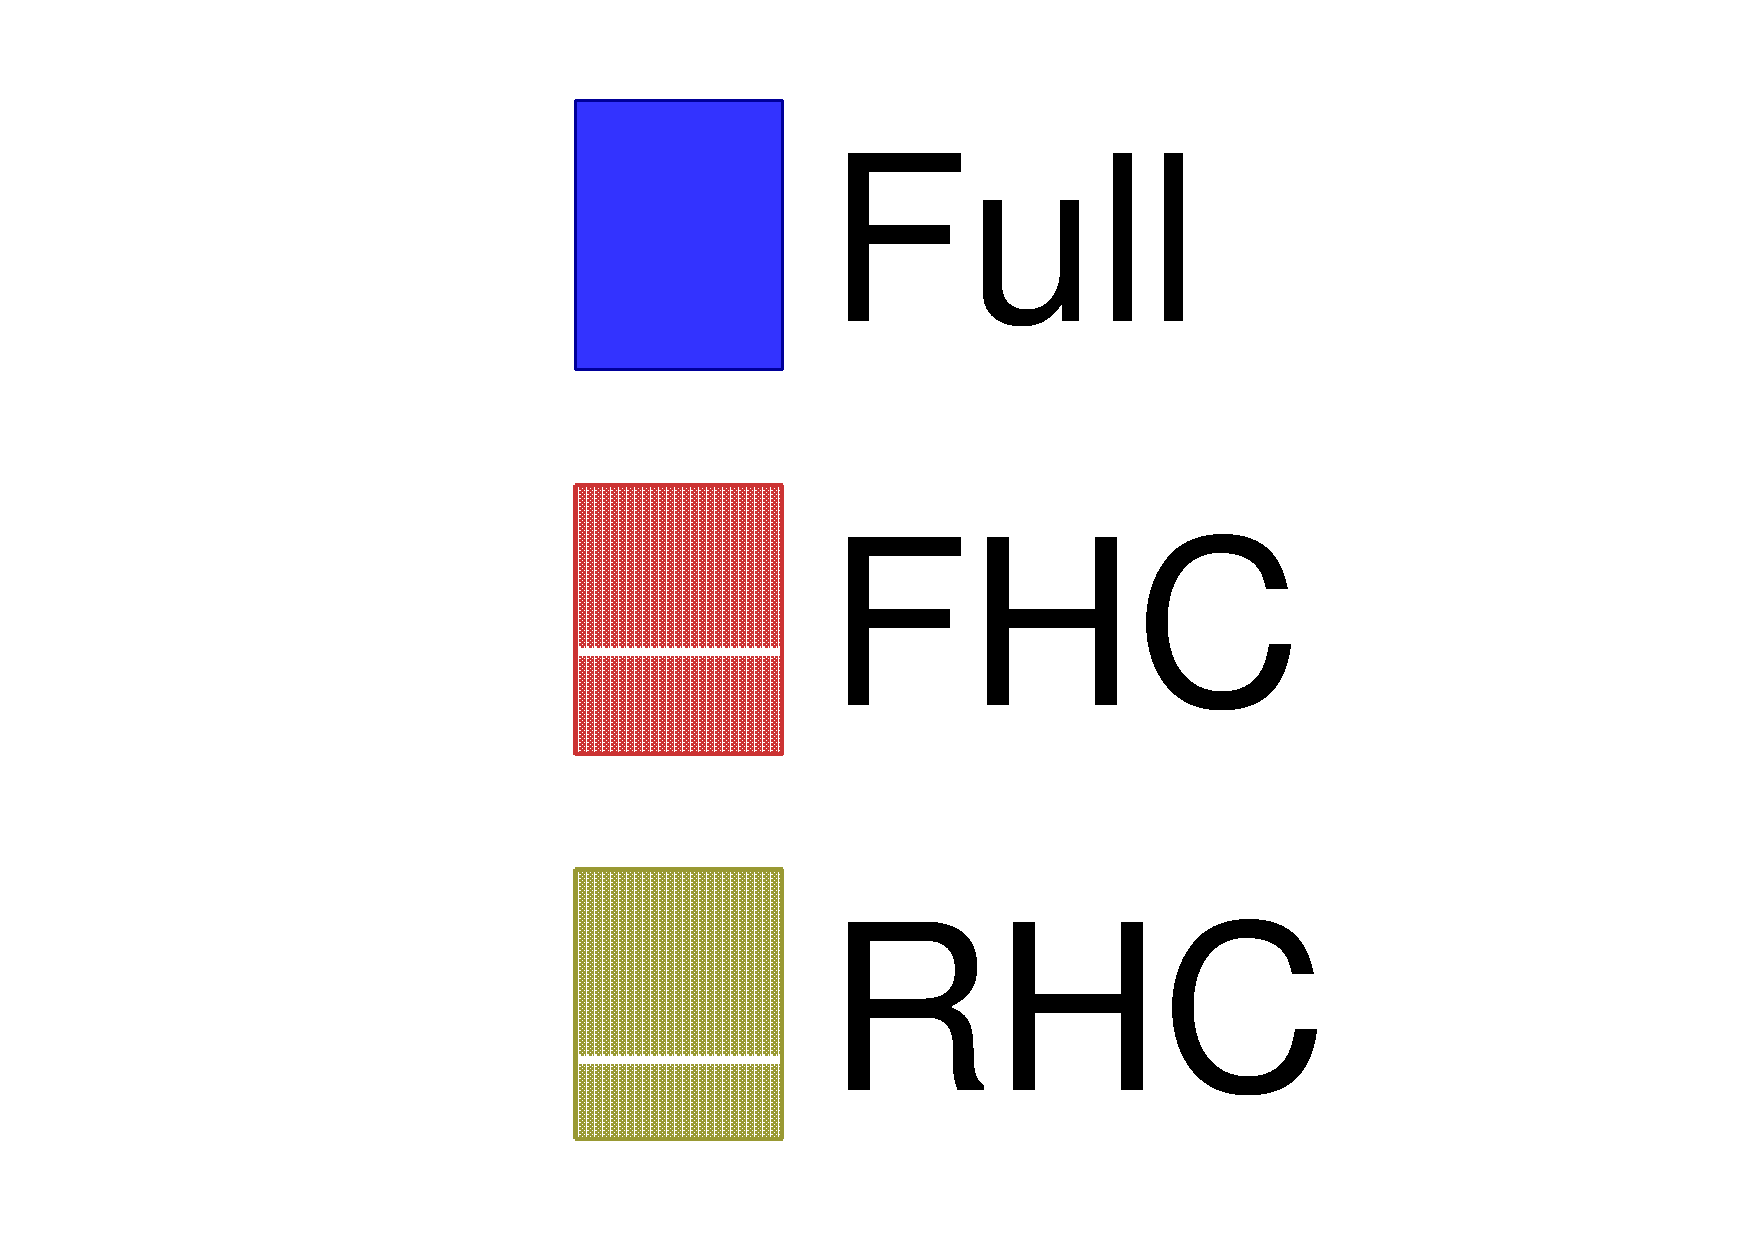
\includegraphics[width=\textwidth, trim={0mm 0mm 0mm 0mm}, clip, page=1]{figures/mach3/data/alt/try_2017_fit_on_sk_spectra_posterior_sk_error_run2to4_spectra_posterior_sk_error_run5to6_spectra}
	\end{subfigure}
	\begin{subfigure}[t]{0.32\textwidth}
		\includegraphics[width=\textwidth, trim={0mm 0mm 0mm 0mm}, clip, page=2]{figures/mach3/data/alt/try_2017_fit_on_sk_spectra_posterior_sk_error_run2to4_spectra_posterior_sk_error_run5to6_spectra}
	\end{subfigure}
	\begin{subfigure}[t]{0.32\textwidth}
		\includegraphics[width=\textwidth, trim={0mm 0mm 0mm 0mm}, clip, page=3]{figures/mach3/data/alt/try_2017_fit_on_sk_spectra_posterior_sk_error_run2to4_spectra_posterior_sk_error_run5to6_spectra}
	\end{subfigure}
	
	\begin{subfigure}[t]{0.32\textwidth}
		\includegraphics[width=\textwidth, trim={0mm 0mm 0mm 0mm}, clip, page=4]{figures/mach3/data/alt/try_2017_fit_on_sk_spectra_posterior_sk_error_run2to4_spectra_posterior_sk_error_run5to6_spectra}
	\end{subfigure}
	\begin{subfigure}[t]{0.32\textwidth}
		\includegraphics[width=\textwidth, trim={0mm 0mm 0mm 0mm}, clip, page=5]{figures/mach3/data/alt/try_2017_fit_on_sk_spectra_posterior_sk_error_run2to4_spectra_posterior_sk_error_run5to6_spectra}
	\end{subfigure}
	\begin{subfigure}[t]{0.32\textwidth}
		\includegraphics[width=\textwidth, trim={0mm 0mm 0mm 0mm}, clip, page=6]{figures/mach3/data/alt/try_2017_fit_on_sk_spectra_posterior_sk_error_run2to4_spectra_posterior_sk_error_run5to6_spectra}
	\end{subfigure}
	
	\caption{Impact of FHC vs RHC fit on SK spectra compared to full fit}
	\label{fig:sk_fhcvsrhc}
\end{figure}

\section{FGD1 vs FGD2}
Reading off \autoref{tab:event_rates_2017} the ratio of FGD1 to FGD2 data is roughly 1, as expected from the detector design. The target in FGD1 is plastic scintillator ($C_8H_8$), whereas FGD2 is alternating layers plastic scintillator and passive water layers. Hence the constraints on $H_2O$ related parameters (e.g. 2p2h shape O) comes purely from FGD2. The location of the TPCs relative each FGD is also important from the view of reconstruction and related systematics: the PID for forward-going tracks is much better in FGD1 due to the two downstream TPCs, whereas FGD2 generally has better backwards going tracking capabilities due to the two upstream TPCs.

\autoref{fig:flux_data_nd280_fdg1vsfgd2} shows the ND280 flux parameters after the fit, in which we mostly similar results for the dominant parameters (correct-sign \numu and \nue). The largest differences happen above $E_\nu=3\text{ GeV}$, where the two fits diverge: FGD2 favouring a much lower flux normalisation at higher energies. The full fit then settles roughtly in between the two fits with an uncertainty covering each individual FGD fit's extreme 1$\sigma$ uncertainty. Interestingly, FGD2 prefers a nominal flux weight at higher $E_\nu$, whereas FGD1 pulls to 0.84. This pattern is repeated for all flux parameters.
\begin{figure}[h]
	\begin{subfigure}[t]{0.10\textwidth}
		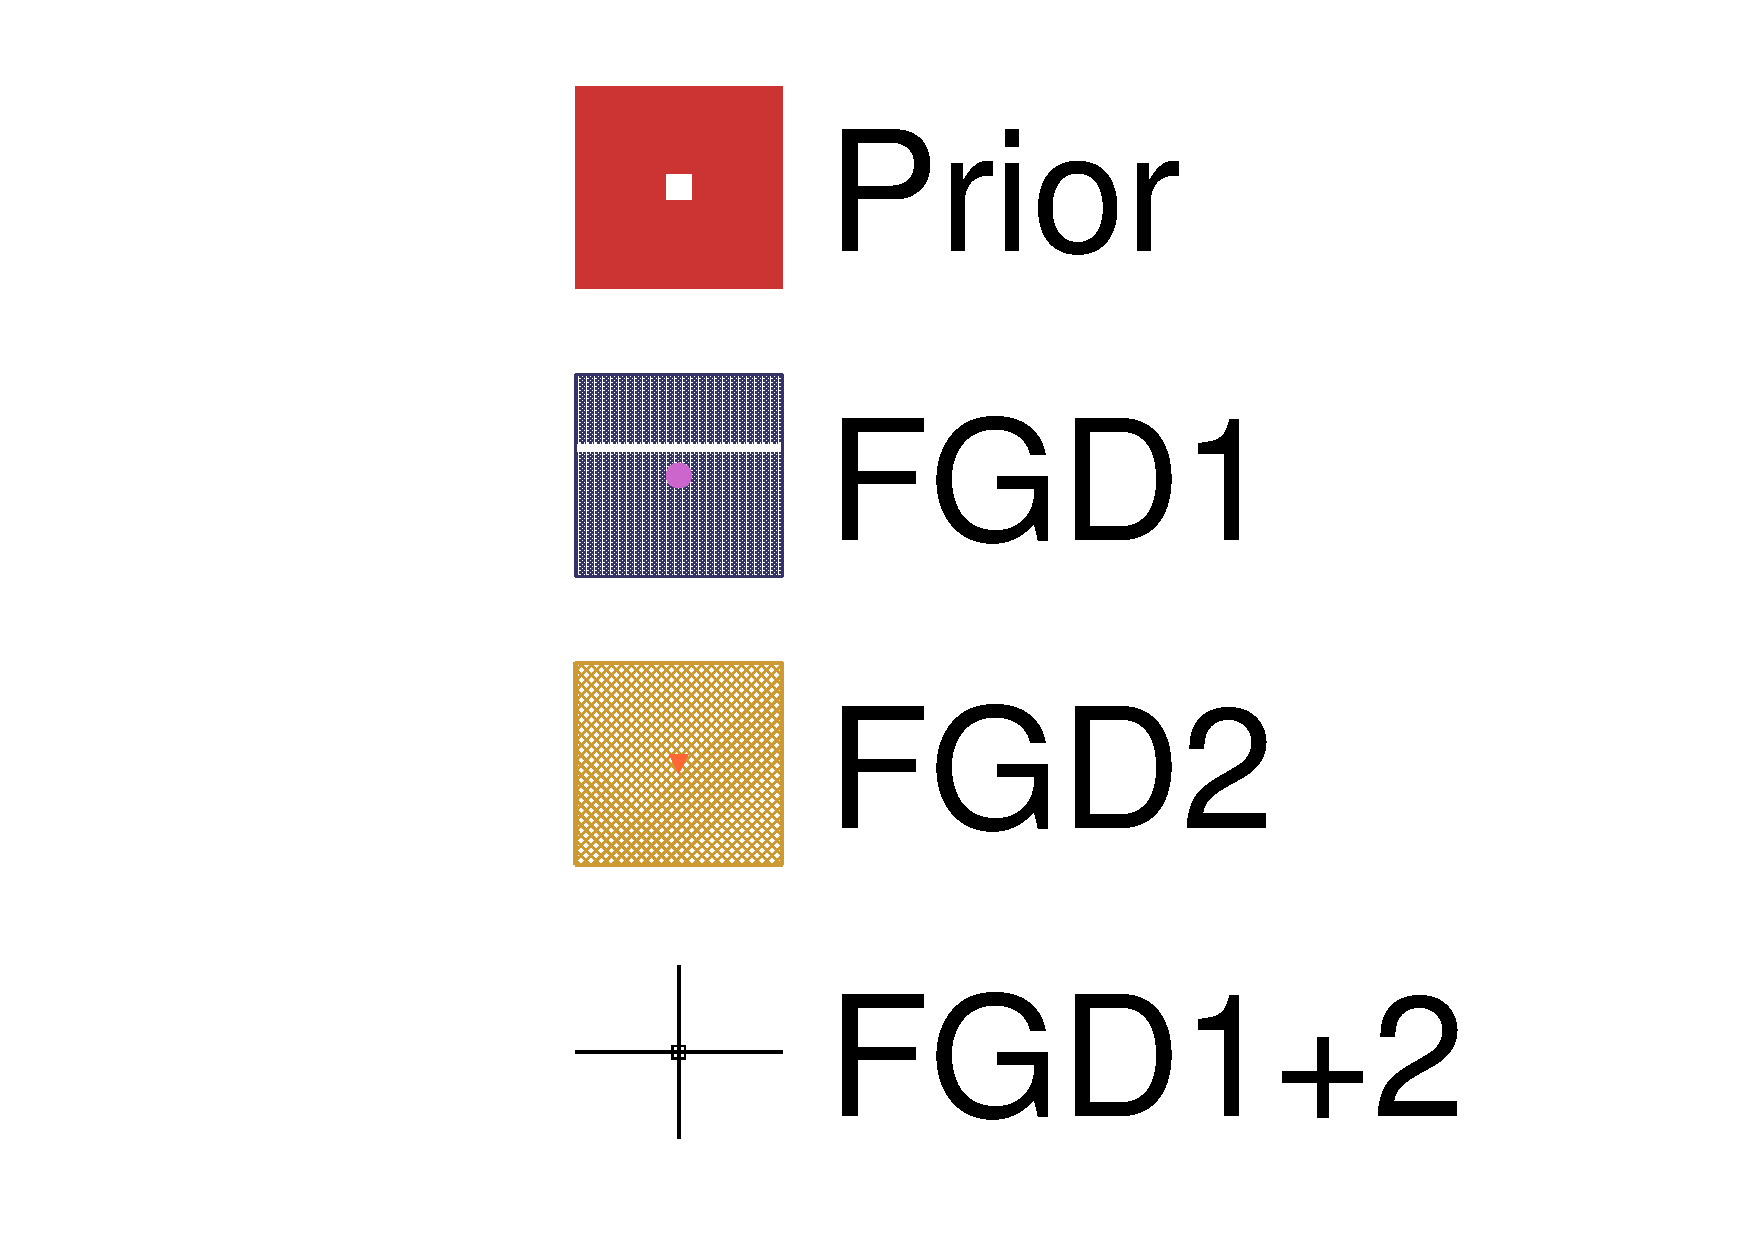
\includegraphics[width=\textwidth, trim={0mm 0mm 0mm 0mm}, clip,page=1]{figures/mach3/data/alt/2017b_FGD1_Data_merge_2017b_FGD2_Data_merge_2017b_NewData_NewDet_UpdXsecStep_2Xsec_4Det_5Flux_0}
	\end{subfigure}
	
	\begin{subfigure}[t]{0.24\textwidth}
		\includegraphics[width=\textwidth, trim={0mm 0mm 0mm 0mm}, clip,page=2]{figures/mach3/data/alt/2017b_FGD1_Data_merge_2017b_FGD2_Data_merge_2017b_NewData_NewDet_UpdXsecStep_2Xsec_4Det_5Flux_0}
	\end{subfigure}
	\begin{subfigure}[t]{0.24\textwidth}
		\includegraphics[width=\textwidth, trim={0mm 0mm 0mm 0mm}, clip,page=3]{figures/mach3/data/alt/2017b_FGD1_Data_merge_2017b_FGD2_Data_merge_2017b_NewData_NewDet_UpdXsecStep_2Xsec_4Det_5Flux_0}
	\end{subfigure}
	\begin{subfigure}[t]{0.24\textwidth}
		\includegraphics[width=\textwidth, trim={0mm 0mm 0mm 0mm}, clip,page=4]{figures/mach3/data/alt/2017b_FGD1_Data_merge_2017b_FGD2_Data_merge_2017b_NewData_NewDet_UpdXsecStep_2Xsec_4Det_5Flux_0}
	\end{subfigure}
	\begin{subfigure}[t]{0.24\textwidth}
		\includegraphics[width=\textwidth, trim={0mm 0mm 0mm 0mm}, clip,page=5]{figures/mach3/data/alt/2017b_FGD1_Data_merge_2017b_FGD2_Data_merge_2017b_NewData_NewDet_UpdXsecStep_2Xsec_4Det_5Flux_0}
	\end{subfigure}
	
	\begin{subfigure}[t]{0.24\textwidth}
		\includegraphics[width=\textwidth, trim={0mm 0mm 0mm 0mm}, clip,page=6]{figures/mach3/data/alt/2017b_FGD1_Data_merge_2017b_FGD2_Data_merge_2017b_NewData_NewDet_UpdXsecStep_2Xsec_4Det_5Flux_0}
	\end{subfigure}
	\begin{subfigure}[t]{0.24\textwidth}
		\includegraphics[width=\textwidth, trim={0mm 0mm 0mm 0mm}, clip,page=7]{figures/mach3/data/alt/2017b_FGD1_Data_merge_2017b_FGD2_Data_merge_2017b_NewData_NewDet_UpdXsecStep_2Xsec_4Det_5Flux_0}
	\end{subfigure}
	\begin{subfigure}[t]{0.24\textwidth}
		\includegraphics[width=\textwidth, trim={0mm 0mm 0mm 0mm}, clip,page=8]{figures/mach3/data/alt/2017b_FGD1_Data_merge_2017b_FGD2_Data_merge_2017b_NewData_NewDet_UpdXsecStep_2Xsec_4Det_5Flux_0}
	\end{subfigure}
	\begin{subfigure}[t]{0.24\textwidth}
		\includegraphics[width=\textwidth, trim={0mm 0mm 0mm 0mm}, clip,page=9]{figures/mach3/data/alt/2017b_FGD1_Data_merge_2017b_FGD2_Data_merge_2017b_NewData_NewDet_UpdXsecStep_2Xsec_4Det_5Flux_0}
	\end{subfigure}
	\caption{ND280 flux parameters after the data fit for FGD1 vs FGD2}
	\label{fig:flux_data_nd280_fdg1vsfgd2}
\end{figure}

\autoref{fig:xsec_data_fdg1vsfgd2} shows the interaction parameters for the fits to individual FGDs. The CC0$\pi$ parameters are mostly in agreement, although there are differences in $M_A^{QE}$ and BeRPA B. For FGD1 $M_A^{QE} = 1.21\pm0.08\text{ GeV}$ , FGD2 $M_A^{QE} = 1.06\pm0.05\text{ GeV}$, and for both $M_A^{QE} = 1.13\pm0.07\text{ GeV}$, so once again the full fit settles between the FGD1 and FGD2 fit. Interestingly, FGD1 fits a similar value of $M_A^{QE}$ to the notorious ``MiniBooNE $M_A^{QE}$ puzzle'' at $M_A^{QE}=1.35\pm0.17\text{ GeV}$ \cite{miniboone_nu_ccqe} (also seen at K2K on oxygen $M_A^{QE}=1.20\pm0.12\text{ GeV}$\cite{k2k_ccqe_oxygen}, at K2K on carbon $M_A^{QE}=1.14\pm0.11\text{ GeV}$\cite{k2k_ccqe_carbon} and MINOS $M_A^{QE}=1.23\pm0.18\text{ GeV}$\cite{minos_ccqe_iron}) , whereas FGD2 fits close to bubble chamber values at $M_A^{QE}=1.069\pm 0.016\text{ GeV}$\cite{maqe_fit}. A slightly lower value of BeRPA B is preferred for the FGD1 only fit, which we may expect from the strong correlation with $M_A^{QE}$. However the full FGD1+2 fit favours a value almost identical to FGD2 alone, with a small decrease in the parameter error.

The CC1$\pi$ parameters are mostly the same with small differences in $C_5^A$ and the coherent normalisation parameters, although they overlap well within eachother's 1$\sigma$ uncertainty. For the FSI parameters, the full data fit tends towards the FGD2 result, and we note slightly larger errors on the FGD1, e.g. for FSI Inel lo.
\begin{figure}[h]
	\begin{subfigure}[t]{0.49\textwidth}
		\includegraphics[width=\textwidth, trim={0mm 0mm 0mm 0mm}, clip,page=18]{figures/mach3/data/alt/2017b_FGD1_Data_merge_2017b_FGD2_Data_merge_2017b_NewData_NewDet_UpdXsecStep_2Xsec_4Det_5Flux_0}
	\end{subfigure}
	\begin{subfigure}[t]{0.49\textwidth}
		\includegraphics[width=\textwidth, trim={0mm 0mm 0mm 0mm}, clip,page=19]{figures/mach3/data/alt/2017b_FGD1_Data_merge_2017b_FGD2_Data_merge_2017b_NewData_NewDet_UpdXsecStep_2Xsec_4Det_5Flux_0}
	\end{subfigure}
	
	\begin{subfigure}[t]{0.49\textwidth}
		\includegraphics[width=\textwidth, trim={0mm 0mm 0mm 0mm}, clip,page=20]{figures/mach3/data/alt/2017b_FGD1_Data_merge_2017b_FGD2_Data_merge_2017b_NewData_NewDet_UpdXsecStep_2Xsec_4Det_5Flux_0}
	\end{subfigure}
	\begin{subfigure}[t]{0.49\textwidth}
		\includegraphics[width=\textwidth, trim={0mm 0mm 0mm 0mm}, clip,page=21]{figures/mach3/data/alt/2017b_FGD1_Data_merge_2017b_FGD2_Data_merge_2017b_NewData_NewDet_UpdXsecStep_2Xsec_4Det_5Flux_0}
	\end{subfigure}
	\caption{Interaction parameters after the data fit for FGD1 vs FGD2}
	\label{fig:xsec_data_fdg1vsfgd2}
\end{figure}

In summary, the two FGDs seem to produce mostly compatible post-fit parameters. The only large difference is the flux normalisation parameters at high $E_\nu$, where FGD1 prefers a much smaller normalisation than FGD2 ($\sim 0.85$ vs $\sim 1.00$). However, this region is very low statistics and barely contributes to the overall event rate at ND280 or SK, so is a small effect in practice. For the interaction parameters we observe slightly different parameters for $M_A^{QE}$ and BeRPA B, in which the fit settles somewhere in between.
% % % % % % % % % % % SK SPECTRA
The FGD1 vs FGD2 fit saw numerous difference in parameters: the high energy flux parameters, $M_A^{QE}$, BeRPA, 2p2h shape and pion absorption parameters all moved within 1$\sigma$ of each other, sometimes on the border.

\autoref{fig:sk_fgd1vsfgd2} shows the predicted oscillated SK event distributions for the three fits, in which all the bins agree well inside each other's 1$\sigma$. The largest deviations are again for the $1\text{R}\mu$ FHC and RHC samples with $0.2 < E_{rec}<0.5\text{ GeV}$, in which the full fit sits higher than the individual fits. The $1\text{R}e$ selection do not show much change.
\begin{figure}[h]
	\begin{subfigure}[t]{0.32\textwidth}
		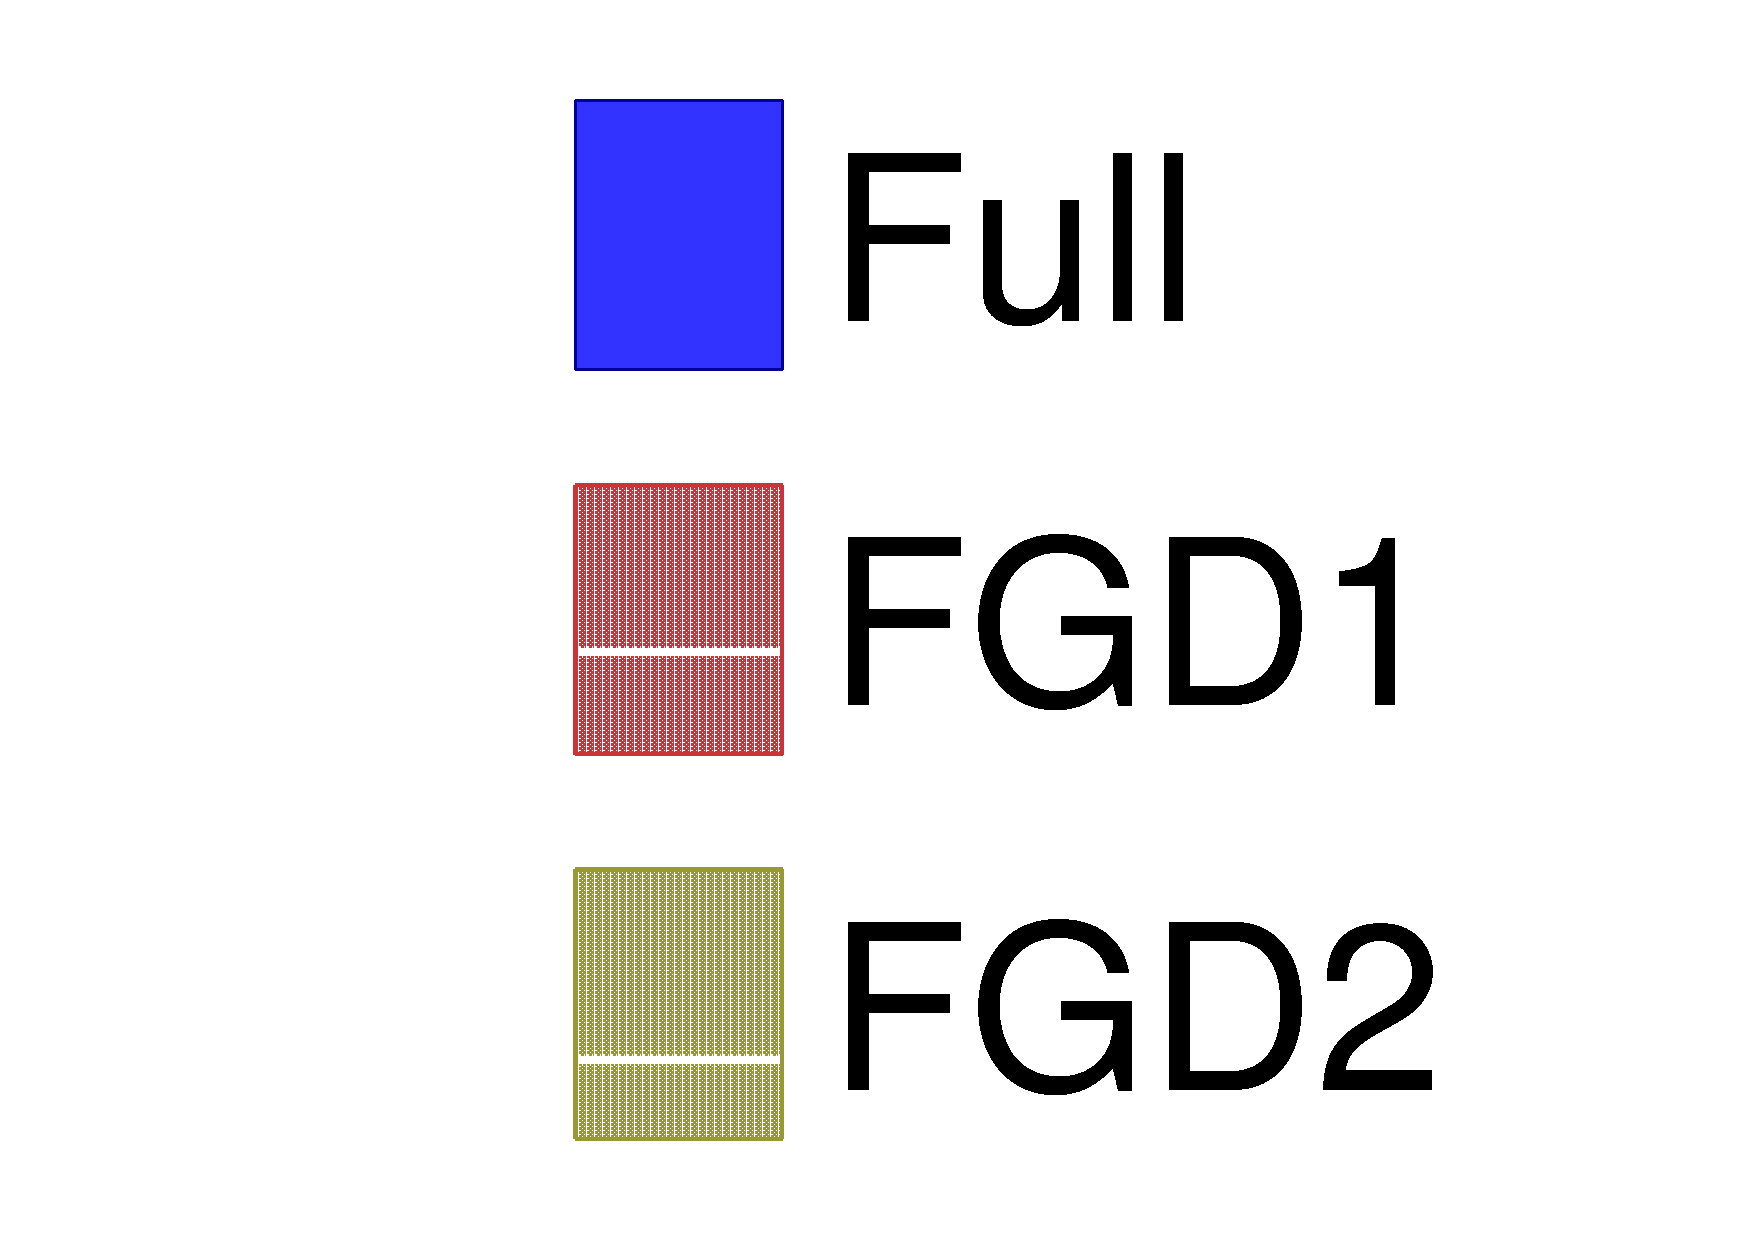
\includegraphics[width=\textwidth, trim={0mm 0mm 0mm 0mm}, clip, page=1]{figures/mach3/data/alt/try_2017_fit_on_sk_spectra_posterior_sk_error_fgd1only_spectra_posterior_sk_error_fgd2only_spectra}
	\end{subfigure}
	\begin{subfigure}[t]{0.32\textwidth}
		\includegraphics[width=\textwidth, trim={0mm 0mm 0mm 0mm}, clip, page=2]{figures/mach3/data/alt/try_2017_fit_on_sk_spectra_posterior_sk_error_fgd1only_spectra_posterior_sk_error_fgd2only_spectra}
	\end{subfigure}
	\begin{subfigure}[t]{0.32\textwidth}
		\includegraphics[width=\textwidth, trim={0mm 0mm 0mm 0mm}, clip, page=3]{figures/mach3/data/alt/try_2017_fit_on_sk_spectra_posterior_sk_error_fgd1only_spectra_posterior_sk_error_fgd2only_spectra}
	\end{subfigure}
	
	\begin{subfigure}[t]{0.32\textwidth}
		\includegraphics[width=\textwidth, trim={0mm 0mm 0mm 0mm}, clip, page=4]{figures/mach3/data/alt/try_2017_fit_on_sk_spectra_posterior_sk_error_fgd1only_spectra_posterior_sk_error_fgd2only_spectra}
	\end{subfigure}
	\begin{subfigure}[t]{0.32\textwidth}
		\includegraphics[width=\textwidth, trim={0mm 0mm 0mm 0mm}, clip, page=5]{figures/mach3/data/alt/try_2017_fit_on_sk_spectra_posterior_sk_error_fgd1only_spectra_posterior_sk_error_fgd2only_spectra}
	\end{subfigure}
	\begin{subfigure}[t]{0.32\textwidth}
		\includegraphics[width=\textwidth, trim={0mm 0mm 0mm 0mm}, clip, page=6]{figures/mach3/data/alt/try_2017_fit_on_sk_spectra_posterior_sk_error_fgd1only_spectra_posterior_sk_error_fgd2only_spectra}
	\end{subfigure}
	\caption{Impact of FGD1 vs FGD2 fit on SK spectra compared to full fit}
	\label{fig:sk_fgd1vsfgd2}
\end{figure}

\section{Excluding the FGD1 CCOther Selection}
The data fit showed a generally good description of the ND280 selections with acceptable p-values and best-fit test-statistics for all but FGD1 CCOther. Here we investigate the impact of the sample on the overall fit with the concern that if some parameterisation of systematics has gone awry it may produce erroneous parameter results propagated to SK. 

The ND280 flux parameters in \autoref{fig:flux_data_nd280_nofgd1ccoth} are almost identical to the full 2017 fit and we note barely any differences: the largest change is 0.015 in the highest $E_\nu$ normalisation of FHC \numu.

\begin{figure}[h]
	\begin{subfigure}[t]{0.10\textwidth}
		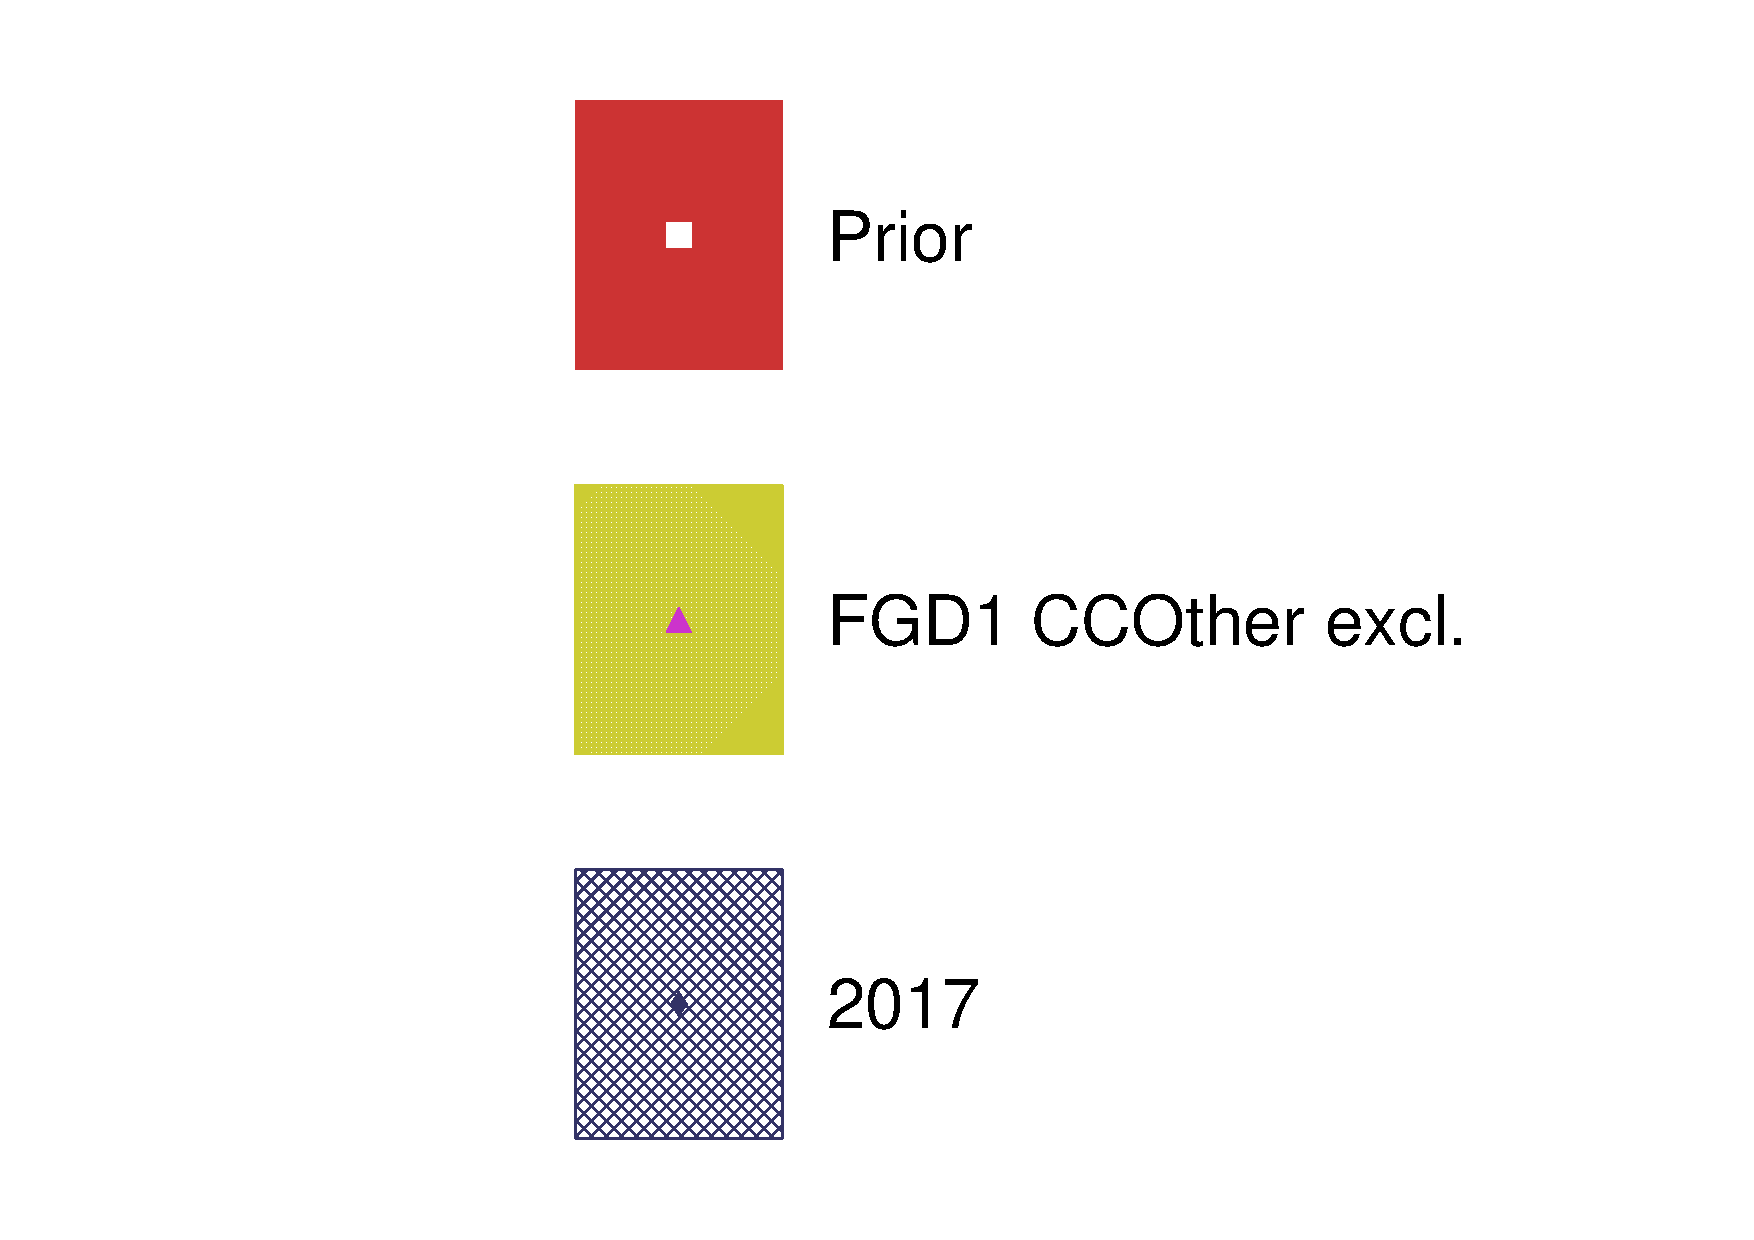
\includegraphics[width=\textwidth, trim={0mm 0mm 0mm 0mm}, clip,page=1]{figures/mach3/data/alt/2017b_NoFGD1CCOth_Data_merg_2017b_NewData_NewDet_UpdXsecStep_2Xsec_4Det_5Flux_0}
	\end{subfigure}
	
	\begin{subfigure}[t]{0.24\textwidth}
		\includegraphics[width=\textwidth, trim={0mm 0mm 0mm 0mm}, clip,page=2]{figures/mach3/data/alt/2017b_NoFGD1CCOth_Data_merg_2017b_NewData_NewDet_UpdXsecStep_2Xsec_4Det_5Flux_0}
	\end{subfigure}
	\begin{subfigure}[t]{0.24\textwidth}
		\includegraphics[width=\textwidth, trim={0mm 0mm 0mm 0mm}, clip,page=3]{figures/mach3/data/alt/2017b_NoFGD1CCOth_Data_merg_2017b_NewData_NewDet_UpdXsecStep_2Xsec_4Det_5Flux_0}
	\end{subfigure}
	\begin{subfigure}[t]{0.24\textwidth}
		\includegraphics[width=\textwidth, trim={0mm 0mm 0mm 0mm}, clip,page=4]{figures/mach3/data/alt/2017b_NoFGD1CCOth_Data_merg_2017b_NewData_NewDet_UpdXsecStep_2Xsec_4Det_5Flux_0}
	\end{subfigure}
	\begin{subfigure}[t]{0.24\textwidth}
		\includegraphics[width=\textwidth, trim={0mm 0mm 0mm 0mm}, clip,page=5]{figures/mach3/data/alt/2017b_NoFGD1CCOth_Data_merg_2017b_NewData_NewDet_UpdXsecStep_2Xsec_4Det_5Flux_0}
	\end{subfigure}
	
	\begin{subfigure}[t]{0.24\textwidth}
		\includegraphics[width=\textwidth, trim={0mm 0mm 0mm 0mm}, clip,page=6]{figures/mach3/data/alt/2017b_NoFGD1CCOth_Data_merg_2017b_NewData_NewDet_UpdXsecStep_2Xsec_4Det_5Flux_0}
	\end{subfigure}
	\begin{subfigure}[t]{0.24\textwidth}
		\includegraphics[width=\textwidth, trim={0mm 0mm 0mm 0mm}, clip,page=7]{figures/mach3/data/alt/2017b_NoFGD1CCOth_Data_merg_2017b_NewData_NewDet_UpdXsecStep_2Xsec_4Det_5Flux_0}
	\end{subfigure}
	\begin{subfigure}[t]{0.24\textwidth}
		\includegraphics[width=\textwidth, trim={0mm 0mm 0mm 0mm}, clip,page=8]{figures/mach3/data/alt/2017b_NoFGD1CCOth_Data_merg_2017b_NewData_NewDet_UpdXsecStep_2Xsec_4Det_5Flux_0}
	\end{subfigure}
	\begin{subfigure}[t]{0.24\textwidth}
		\includegraphics[width=\textwidth, trim={0mm 0mm 0mm 0mm}, clip,page=9]{figures/mach3/data/alt/2017b_NoFGD1CCOth_Data_merg_2017b_NewData_NewDet_UpdXsecStep_2Xsec_4Det_5Flux_0}
	\end{subfigure}
	\caption{ND280 flux parameters after the data fit for excluding FGD1 CCOther}
	\label{fig:flux_data_nd280_nofgd1ccoth}
\end{figure}

The interaction parameters in \autoref{fig:xsec_data_nofgd1ccoth} shows slightly more change in the single and multi-pion related parameters, although the CC0$\pi$ parameters remain unchanged. The changes happen in the poorly constrained non-resonant $I_{1/2}$ background parameter, the CC DIS parameter, and some of the FSI parameters. All the differences are however well within the full data fit result.
\begin{figure}[h]
	\begin{subfigure}[t]{0.49\textwidth}
		\includegraphics[width=\textwidth, trim={0mm 0mm 0mm 0mm}, clip,page=18]{figures/mach3/data/alt/2017b_NoFGD1CCOth_Data_merg_2017b_NewData_NewDet_UpdXsecStep_2Xsec_4Det_5Flux_0}
	\end{subfigure}
	\begin{subfigure}[t]{0.49\textwidth}
		\includegraphics[width=\textwidth, trim={0mm 0mm 0mm 0mm}, clip,page=19]{figures/mach3/data/alt/2017b_NoFGD1CCOth_Data_merg_2017b_NewData_NewDet_UpdXsecStep_2Xsec_4Det_5Flux_0}
	\end{subfigure}
	
	\begin{subfigure}[t]{0.49\textwidth}
		\includegraphics[width=\textwidth, trim={0mm 0mm 0mm 0mm}, clip,page=20]{figures/mach3/data/alt/2017b_NoFGD1CCOth_Data_merg_2017b_NewData_NewDet_UpdXsecStep_2Xsec_4Det_5Flux_0}
	\end{subfigure}
	\begin{subfigure}[t]{0.49\textwidth}
		\includegraphics[width=\textwidth, trim={0mm 0mm 0mm 0mm}, clip,page=21]{figures/mach3/data/alt/2017b_NoFGD1CCOth_Data_merg_2017b_NewData_NewDet_UpdXsecStep_2Xsec_4Det_5Flux_0}
	\end{subfigure}
	\caption{Interaction parameters after the data fit for excluding FGD1 CCOther}
	\label{fig:xsec_data_nofgd1ccoth}
\end{figure}

The event rate and $-2\ln\mathcal{L}_s$ for including and excluding FGD1 CCOther is shown in \autoref{tab:postfit_eventrate_nofgd1ccother} and as expected there is no greater difference between the two fits in central values or uncertainties: the total difference across all samples is 50.5 events and for the test-statistic it's 2.25.
\begin{table}[h]
	\centering
	\begin{tabular}{ l | c c | c c }
		\hline
		\hline
		Sample 		& \multicolumn{2}{c|}{Event rate} & \multicolumn{2}{c}{$-2\ln{\mathcal{L}_s}$} \\
		& 2017 & FGD1 CCOth & 2017 & FGD1 CCOth\\
		\hline
		FGD1 0$\pi$ 	& $17122.9\pm120.0$ & $17121.6\pm120.9$ & 172.21  & 170.75 \\ 
		FGD1 1$\pi$ 	& $4053.8\pm54.3$   & $4032.4\pm54.0$ & 164.04 & 162.14	\\ 
		\hline
		FGD2 0$\pi$ 	& $17501.5\pm122.5$ & $17487.9\pm121.4$ & 166.15  & 166.28 \\ 
		FGD2 1$\pi$ 	& $3409.4\pm48.2$   & $3408.7\pm46.1$ &  162.71 & 162.26	\\ 
		FGD2 Other 	& $3917.8\pm50.8$  & $3906.6\pm55.8$ & 171.17 & 172.05	\\ 
		\hline
		FGD1 1Trk 	& $3509.6\pm50.1$  & $3513.1\pm50.1$ & 117.80 &117.15	\\ 
		FGD1 NTrk 	& $1062.7\pm21.9$  & $1046.7\pm23.6$ & 76.50 	& 76.36\\ 
		FGD2 1Trk 	& $3678.7\pm51.3$  & $3679.0\pm53.0$ & 129.84 	& 128.44 \\ 
		FGD2 NTrk 	& $1108.4\pm23.5$  & $1105.1\pm19.8$ & 80.34 	& 80.72 \\ 
		\hline
		FGD1 \numu 1Trk & $1348.3\pm23.1$  & $1351.6\pm24.5$ & 66.51 	& 66.38 \\
		FGD1 \numu NTrk & $1359.1\pm26.9$  & $1351.4\pm26.0$ & 61.75 	& 61.17 \\
		FGD2 \numu 1Trk & $1323.1\pm23.8$  & $1327.6\pm23.3$ & 64.34 	& 65.09 \\
		FGD2 \numu NTrk	& $1265.9\pm24.2$  & $1272.3\pm25.1$ & 75.70 	& 78.00 \\
		\hline
		Total 		& $60658.1$ & $60607.6\pm244.1$ & 1509.05 & 1506.81 \\ 
		\hline
		\hline
	\end{tabular}
	\caption{Event rate and test-statistic for 2017 with and without FGD1 CCOther. N.B. the total rate and test-statistic for 2017 has the values for FGD1 CCOther subtracted}
	\label{tab:postfit_eventrate_nofgd1ccother}
\end{table}

Finally we recalculate the sample-by-sample p-values in \autoref{tab:data_post_pvalue_nofgd1ccother} for direct comparison to the full data fit values in \autoref{tab:data_post_pvalue}. The difference between the two fits' posterior predictive p-values is maximally 7\% for FGD2 NTrk (from 58.7\% to 51.7\%) and all p-values are deemed acceptable.
\begin{table}[h]
	\centering
	\begin{tabular}{l | c c }
		\hline \hline
		Sample & Draw Fluc. & Pred. Fluc. \\
		\hline
		FGD1 0$\pi$ & 0.075 & 0.071 \\
		FGD1 1$\pi$ & 0.089 & 0.086 \\
		FGD2 0$\pi$ & 0.113 & 0.115 \\
		FGD2 1$\pi$ & 0.087 & 0.096 \\
		FGD2 Other  & 0.090 & 0.087 \\
		\hline
		FGD1 1Trk & 0.526 & 0.529 \\
		FGD1 NTrk & 0.293 & 0.281 \\
		FGD2 1Trk & 0.293 & 0.288 \\
		FGD2 NTrk & 0.208 & 0.206 \\
		\hline
		FGD1 \numu 1Trk & 0.283 & 0.287 \\
		FGD1 \numu NTrk & 0.860 & 0.859 \\
		FGD2 \numu 1Trk & 0.313 & 0.307 \\
		FGD2 \numu NTrk & 0.517 & 0.520 \\
		\hline
		\hline
	\end{tabular}
	\caption{Posterior predictive p-values for each sample after the data fit excluding FGD1 CCOther}
	\label{tab:data_post_pvalue_nofgd1ccother}
\end{table}

\section{Using a 2015-like Model}
The 2017 oscillation analysis saw numerous updates to the cross-section model which attempted to provide freedom to nuclear effects such as multi-nucleon interactions and RPA corrections. Ideally, the flux and interaction model is moving closer towards reality than being an ``effective'' model, being able to only describe ND280-like detectors in a flux similar to that at ND280. 

In this section we compare the parameter values from the 2017 analysis to a modified 2017 model made to resemble that of 2015 \cite{t2k_2015}. In 2015 there was no freedom to change the 2p2h shape or the RPA correction, which was at the time thought to be a weakness in the analysis. The 2p2h normalisation were applied, albeit in a different fashion where 2p2h norm $\bar{\nu}$ was applied multiplicatively to the 2p2h norm $\nu$ weight for $\bar{\nu}$ 2p2h events, effectively correlating the parameters. The 2p2h normalisation was also separated for Carbon and Oxygen, but were found to be the same after the fit. For the 2017 analysis these parameters are uncorrelated. The priors on the single pion parameters changed slightly too, but overall only shifted central values by small amounts and gave larger uncertainties on the prior.

A straight-forward implementation of the 2015 cross-section model is therefore to fix 2p2h shape C and O and the BeRPA parameters to their nominal values and not vary them during the fit. Here we compare such a model to the results of the full data fit, drawing parallels with the 2015 results.

\autoref{fig:2015_fluxND280comp_fhc} and \autoref{fig:2015_fluxND280comp_rhc} shows the ND280 flux parameters for the two fits, including the result from 2015. \cite{t2k_2015}. The 2015-like fit result replicates the main feature of the 2015 fit: the notably high normalisation of $\sim10-20\%$ throughout the flux parameters. However, it does not perfectly replicate the parameter results, as the dip for the 2017 result for FHC \numu around $E_\nu = 0.8-1.0\text{ GeV}$ is also present in the 2015-like fit, but not in the actual 2015 fit. The RHC parameters for the 2015-like fit in \autoref{fig:2015_fluxND280comp_rhc} agree more with the 2015 result with the key features replicated.

\begin{figure}[h]
	\begin{subfigure}[t]{0.10\textwidth}
		\includegraphics[width=\textwidth, trim={0mm 0mm 0mm 0mm}, clip,page=1]{figures/mach3/data/alt/2017b_NewData_NewDet_hpc_2015like__2017b_NewData_NewDet_UpdXsecStep_2Xsec_4Det_5Flux_0.pdf}
	\end{subfigure}
	
	\begin{subfigure}[t]{\textwidth}
		\begin{subfigure}[t]{0.24\textwidth}
			\includegraphics[width=\textwidth, trim={0mm 0mm 0mm 0mm}, clip,page=2]{figures/mach3/data/alt/2017b_NewData_NewDet_hpc_2015like__2017b_NewData_NewDet_UpdXsecStep_2Xsec_4Det_5Flux_0.pdf}
		\end{subfigure}
		\begin{subfigure}[t]{0.24\textwidth}
			\includegraphics[width=\textwidth, trim={0mm 0mm 0mm 0mm}, clip,page=3]{figures/mach3/data/alt/2017b_NewData_NewDet_hpc_2015like__2017b_NewData_NewDet_UpdXsecStep_2Xsec_4Det_5Flux_0.pdf}
		\end{subfigure}
		\begin{subfigure}[t]{0.24\textwidth}
			\includegraphics[width=\textwidth, trim={0mm 0mm 0mm 0mm}, clip,page=4]{figures/mach3/data/alt/2017b_NewData_NewDet_hpc_2015like__2017b_NewData_NewDet_UpdXsecStep_2Xsec_4Det_5Flux_0.pdf}
		\end{subfigure}
		\begin{subfigure}[t]{0.24\textwidth}
			\includegraphics[width=\textwidth, trim={0mm 0mm 0mm 0mm}, clip,page=5]{figures/mach3/data/alt/2017b_NewData_NewDet_hpc_2015like__2017b_NewData_NewDet_UpdXsecStep_2Xsec_4Det_5Flux_0.pdf}
		\end{subfigure}
		\caption{2017 and 2015-like}
	\end{subfigure}
	
	\begin{subfigure}[t]{\textwidth}
		\begin{subfigure}[t]{0.24\textwidth}
			\includegraphics[width=\textwidth, trim={0mm 0mm 20mm 0mm}, clip]{figures/official/nd_pf_numu_flux_parms_bias_01}
		\end{subfigure}
		\begin{subfigure}[t]{0.24\textwidth}
			\includegraphics[width=\textwidth, trim={0mm 0mm 20mm 0mm}, clip]{figures/official/nd_pf_nue_flux_parms_bias_01}
		\end{subfigure}
		\begin{subfigure}[t]{0.24\textwidth}
			\includegraphics[width=\textwidth, trim={0mm 0mm 20mm 0mm}, clip]{figures/official/nd_pf_numub_flux_parms_bias_01}
		\end{subfigure}
		\begin{subfigure}[t]{0.24\textwidth}
			\includegraphics[width=\textwidth, trim={0mm 0mm 20mm 0mm}, clip]{figures/official/nd_pf_nueb_flux_parms_bias_01}
		\end{subfigure}
		\caption{2015 results}
	\end{subfigure}
	
	\caption{ND280 FHC flux parameters for 2017, 2015-like and 2015 analyses}
	\label{fig:2015_fluxND280comp_fhc}
\end{figure}

\begin{figure}[h]
	\begin{subfigure}[t]{\textwidth}
		\begin{subfigure}[t]{0.24\textwidth}
			\includegraphics[width=\textwidth, trim={0mm 0mm 0mm 0mm}, clip,page=6]{figures/mach3/data/alt/2017b_NewData_NewDet_hpc_2015like__2017b_NewData_NewDet_UpdXsecStep_2Xsec_4Det_5Flux_0.pdf}
		\end{subfigure}
		\begin{subfigure}[t]{0.24\textwidth}
			\includegraphics[width=\textwidth, trim={0mm 0mm 0mm 0mm}, clip,page=7]{figures/mach3/data/alt/2017b_NewData_NewDet_hpc_2015like__2017b_NewData_NewDet_UpdXsecStep_2Xsec_4Det_5Flux_0.pdf}
		\end{subfigure}
		\begin{subfigure}[t]{0.24\textwidth}
			\includegraphics[width=\textwidth, trim={0mm 0mm 0mm 0mm}, clip,page=8]{figures/mach3/data/alt/2017b_NewData_NewDet_hpc_2015like__2017b_NewData_NewDet_UpdXsecStep_2Xsec_4Det_5Flux_0.pdf}
		\end{subfigure}
		\begin{subfigure}[t]{0.24\textwidth}
			\includegraphics[width=\textwidth, trim={0mm 0mm 0mm 0mm}, clip,page=9]{figures/mach3/data/alt/2017b_NewData_NewDet_hpc_2015like__2017b_NewData_NewDet_UpdXsecStep_2Xsec_4Det_5Flux_0.pdf}
		\end{subfigure}
		\caption{2017 and 2015-like}
	\end{subfigure}
	
	\begin{subfigure}[t]{\textwidth}
		\begin{subfigure}[t]{0.24\textwidth}
			\includegraphics[width=\textwidth, trim={0mm 0mm 20mm 0mm}, clip]{figures/official/nd_nf_numub_flux_parms_bias_01}
		\end{subfigure}
		\begin{subfigure}[t]{0.24\textwidth}
			\includegraphics[width=\textwidth, trim={0mm 0mm 20mm 0mm}, clip]{figures/official/nd_nf_nueb_flux_parms_bias_01}
		\end{subfigure}
		\begin{subfigure}[t]{0.24\textwidth}
			\includegraphics[width=\textwidth, trim={0mm 0mm 20mm 0mm}, clip]{figures/official/nd_nf_numu_flux_parms_bias_01}
		\end{subfigure}
		\begin{subfigure}[t]{0.24\textwidth}
			\includegraphics[width=\textwidth, trim={0mm 0mm 20mm 0mm}, clip]{figures/official/nd_nf_nue_flux_parms_bias_01}
		\end{subfigure}
		\caption{2015 results}
	\end{subfigure}
	\caption{ND280 RHC flux parameters for 2017, 2015-like and 2015 analyses}
	\label{fig:2015_fluxND280comp_rhc}
\end{figure}

\autoref{fig:xsec_data_2015like} show the interaction parameters, in which we note a similar values for the directly comparable parameters, e.g. $M_A^{QE}$, $p_F$, $C_5^A$, CC DIS, NC other.  We also note the difference in the CC DIS parameter, which moves from nominal (2015 and 2015-like) to roughly its upper $1\sigma$. Since the CC DIS parameter is heavily connected to an event's $E_\nu$ (since the parameter is $0.4/E_\nu$), this is likely a reflection of the central values of the fluxes shifting from $\sim1.1$ to $\sim1.0$ in moving from the 2015 to 2017 analysis.
\begin{figure}[h]
	\begin{subfigure}[t]{\textwidth}
		\begin{subfigure}[t]{0.24\textwidth}
			\includegraphics[width=\textwidth, trim={0mm 0mm 0mm 0mm}, clip,page=18]{figures/mach3/data/alt/2017b_NewData_NewDet_hpc_2015like__2017b_NewData_NewDet_UpdXsecStep_2Xsec_4Det_5Flux_0.pdf}
		\end{subfigure}
		\begin{subfigure}[t]{0.24\textwidth}
			\includegraphics[width=\textwidth, trim={0mm 0mm 0mm 0mm}, clip,page=19]{figures/mach3/data/alt/2017b_NewData_NewDet_hpc_2015like__2017b_NewData_NewDet_UpdXsecStep_2Xsec_4Det_5Flux_0.pdf}
		\end{subfigure}
		\begin{subfigure}[t]{0.24\textwidth}
			\includegraphics[width=\textwidth, trim={0mm 0mm 0mm 0mm}, clip,page=20]{figures/mach3/data/alt/2017b_NewData_NewDet_hpc_2015like__2017b_NewData_NewDet_UpdXsecStep_2Xsec_4Det_5Flux_0.pdf}
		\end{subfigure}
		\begin{subfigure}[t]{0.24\textwidth}
			\includegraphics[width=\textwidth, trim={0mm 0mm 0mm 0mm}, clip,page=21]{figures/mach3/data/alt/2017b_NewData_NewDet_hpc_2015like__2017b_NewData_NewDet_UpdXsecStep_2Xsec_4Det_5Flux_0.pdf}
		\end{subfigure}
		\caption{2017 and 2015-like}
	\end{subfigure}
	
	\begin{subfigure}[t]{\textwidth}
		\centering
		\begin{subfigure}[t]{0.5\textwidth}
			\includegraphics[width=\textwidth, trim={0mm 0mm 0mm 0mm}, clip]{figures/official/banff_data_paramplot_20160408_03.pdf}
		\end{subfigure}
		\caption{2015 results}
	\end{subfigure}
	
	\caption{Interaction parameters for 2017, 2015-like and 2015 analyses}
	\label{fig:xsec_data_2015like}
\end{figure}

\paragraph{A Model with BeRPA and 2p2h Shape Fixed}
From the initial likelihood scans and 1$\sigma$ variations to the Asimov data set in \autoref{sec:llh_scan} and \autoref{sec:sigmavar}, it is expected that the ``2015-like'' quality of keeping BeRPA and 2p2h shape parameters fixed comes from the BeRPA variation. But both BeRPA and 2p2h shape are pulled away from the nominal correction, which the scans and parameter variations were centralised on. Two additional MCMCs were run on the data with variations of the 2015-like cross-section model: fixing the BeRPA parameters at nominal and leaving 2p2h shape free, and vice versa. 

\autoref{fig:2015like_berpa_2p2h_comp_flux} shows the flux parameters after the fits for the different variations and confirms suspicions that the BeRPA parameters are causing the shift in flux parameters. Fixing 2p2h shape to their nominal values has a minor impact on the flux parameters and narrowly replicates the 2015-like fit.
\begin{figure}[h]
	\begin{subfigure}[t]{0.1\textwidth}
		\includegraphics[width=\textwidth, trim={0mm 0mm 0mm 0mm}, clip,page=1]{figures/mach3/data/alt/2017b_NewData_NewDet_hpc_2p2hshapeFix_0_2017b_NewData_NewDet_hpc_BeRPAfix_0_2017b_NewData_NewDet_hpc_2015like_0.pdf}
	\end{subfigure}
	
	\begin{subfigure}[t]{0.24\textwidth}
		\includegraphics[width=\textwidth, trim={0mm 0mm 0mm 0mm}, clip,page=2]{figures/mach3/data/alt/2017b_NewData_NewDet_hpc_2p2hshapeFix_0_2017b_NewData_NewDet_hpc_BeRPAfix_0_2017b_NewData_NewDet_hpc_2015like_0.pdf}
	\end{subfigure}
	\begin{subfigure}[t]{0.24\textwidth}
		\includegraphics[width=\textwidth, trim={0mm 0mm 0mm 0mm}, clip,page=3]{figures/mach3/data/alt/2017b_NewData_NewDet_hpc_2p2hshapeFix_0_2017b_NewData_NewDet_hpc_BeRPAfix_0_2017b_NewData_NewDet_hpc_2015like_0.pdf}
	\end{subfigure}
	\begin{subfigure}[t]{0.24\textwidth}
		\includegraphics[width=\textwidth, trim={0mm 0mm 0mm 0mm}, clip,page=4]{figures/mach3/data/alt/2017b_NewData_NewDet_hpc_2p2hshapeFix_0_2017b_NewData_NewDet_hpc_BeRPAfix_0_2017b_NewData_NewDet_hpc_2015like_0.pdf}
	\end{subfigure}
	\begin{subfigure}[t]{0.24\textwidth}
		\includegraphics[width=\textwidth, trim={0mm 0mm 0mm 0mm}, clip,page=5]{figures/mach3/data/alt/2017b_NewData_NewDet_hpc_2p2hshapeFix_0_2017b_NewData_NewDet_hpc_BeRPAfix_0_2017b_NewData_NewDet_hpc_2015like_0.pdf}
	\end{subfigure}
	
	\begin{subfigure}[t]{0.24\textwidth}
		\includegraphics[width=\textwidth, trim={0mm 0mm 0mm 0mm}, clip,page=6]{figures/mach3/data/alt/2017b_NewData_NewDet_hpc_2p2hshapeFix_0_2017b_NewData_NewDet_hpc_BeRPAfix_0_2017b_NewData_NewDet_hpc_2015like_0.pdf}
	\end{subfigure}
	\begin{subfigure}[t]{0.24\textwidth}
		\includegraphics[width=\textwidth, trim={0mm 0mm 0mm 0mm}, clip,page=7]{figures/mach3/data/alt/2017b_NewData_NewDet_hpc_2p2hshapeFix_0_2017b_NewData_NewDet_hpc_BeRPAfix_0_2017b_NewData_NewDet_hpc_2015like_0.pdf}
	\end{subfigure}
	\begin{subfigure}[t]{0.24\textwidth}
		\includegraphics[width=\textwidth, trim={0mm 0mm 0mm 0mm}, clip,page=8]{figures/mach3/data/alt/2017b_NewData_NewDet_hpc_2p2hshapeFix_0_2017b_NewData_NewDet_hpc_BeRPAfix_0_2017b_NewData_NewDet_hpc_2015like_0.pdf}
	\end{subfigure}
	\begin{subfigure}[t]{0.24\textwidth}
		\includegraphics[width=\textwidth, trim={0mm 0mm 0mm 0mm}, clip,page=9]{figures/mach3/data/alt/2017b_NewData_NewDet_hpc_2p2hshapeFix_0_2017b_NewData_NewDet_hpc_BeRPAfix_0_2017b_NewData_NewDet_hpc_2015like_0.pdf}
	\end{subfigure}
	\caption{Flux parameters for 2015-like, 2p2h shape fixed and BeRPA fixed models}
	\label{fig:2015like_berpa_2p2h_comp_flux}
\end{figure}

\autoref{fig:2015like_berpa_2p2h_comp_xsec} shows the cross-section parameters for the 2015-like variations and we notice much the same pattern. All the observable differences are in 2p2h normalisations, $C_5^A$ and CC DIS all come from the difference in the flux parameter's central values.
\begin{figure}[h]
	\begin{subfigure}[t]{0.49\textwidth}
		\includegraphics[width=\textwidth, trim={0mm 0mm 0mm 0mm}, clip,page=18]{figures/mach3/data/alt/2017b_NewData_NewDet_hpc_2p2hshapeFix_0_2017b_NewData_NewDet_hpc_BeRPAfix_0_2017b_NewData_NewDet_hpc_2015like_0.pdf}
	\end{subfigure}
	\begin{subfigure}[t]{0.49\textwidth}
		\includegraphics[width=\textwidth, trim={0mm 0mm 0mm 0mm}, clip,page=19]{figures/mach3/data/alt/2017b_NewData_NewDet_hpc_2p2hshapeFix_0_2017b_NewData_NewDet_hpc_BeRPAfix_0_2017b_NewData_NewDet_hpc_2015like_0.pdf}
	\end{subfigure}
	
	\begin{subfigure}[t]{0.49\textwidth}
		\includegraphics[width=\textwidth, trim={0mm 0mm 0mm 0mm}, clip,page=20]{figures/mach3/data/alt/2017b_NewData_NewDet_hpc_2p2hshapeFix_0_2017b_NewData_NewDet_hpc_BeRPAfix_0_2017b_NewData_NewDet_hpc_2015like_0.pdf}
	\end{subfigure}
	\begin{subfigure}[t]{0.49\textwidth}
		\includegraphics[width=\textwidth, trim={0mm 0mm 0mm 0mm}, clip,page=21]{figures/mach3/data/alt/2017b_NewData_NewDet_hpc_2p2hshapeFix_0_2017b_NewData_NewDet_hpc_BeRPAfix_0_2017b_NewData_NewDet_hpc_2015like_0.pdf}
	\end{subfigure}
	\caption{Interaction parameters for 2015-like, 2p2h shape fixed and BeRPA fixed models}
	\label{fig:2015like_berpa_2p2h_comp_xsec}
\end{figure}

In summary, it appears that the 2017 analysis agreeing with the flux parameter is down to moving freedom from $E_\nu$ normalisations (the flux parameters) to $Q_2$ normalisations (the BeRPA parameters). Although the BeRPA parametrisation's post-fit model is a strong distortion of the nominal RPA model---implying the parameterisation of the error should be reconsidered---it is more justified assigning error to BeRPA (which has no external data constraints) than the flux model (which has multitudes of external data and monitoring systems).

% % % % % % % % % % % % SK SPECTRA
The 2015-like parameterisation fixed 2p2h shape and BeRPA to their prior values and did not vary them in the fit. This roughly reproduced the results from the ND280 fit from 2015\cite{t2k_2015}. 

\autoref{fig:sk_2015like} shows the $E_{reco}$ distributions for the five samples at Super-Kamiokande. We note the largest difference in spectrum is in the $1\text{R}\mu$ sample between $0.2 < E_{rec} < 0.5\text{ GeV}$: the region which is sensitive to oscillation parameters (mostly $\theta_{23}$ and $\Delta m^2_{23}$ or $\Delta m^2_{32}$). The shift is less than 1$\sigma$ of the full data fit. The $1\text{R}e$ selection has a consistently lower event rate for the 2015-like fit, which has an impact on $\theta_{13}$ primarily, and the effect on the $1\text{R}e1\text{d}e$ selection is opposite. The RHC selections are entirely consistent and see no deviations from each other.
\begin{figure}[h]
	\begin{subfigure}[t]{0.32\textwidth}
		\includegraphics[width=\textwidth, trim={0mm 0mm 0mm 0mm}, clip, page=1]{figures/mach3/data/alt/try_2017_fit_on_sk_spectra_posterior_sk_error_2015like_spectra}
	\end{subfigure}
	\begin{subfigure}[t]{0.32\textwidth}
		\includegraphics[width=\textwidth, trim={0mm 0mm 0mm 0mm}, clip, page=2]{figures/mach3/data/alt/try_2017_fit_on_sk_spectra_posterior_sk_error_2015like_spectra}
	\end{subfigure}
	\begin{subfigure}[t]{0.32\textwidth}
		\includegraphics[width=\textwidth, trim={0mm 0mm 0mm 0mm}, clip, page=3]{figures/mach3/data/alt/try_2017_fit_on_sk_spectra_posterior_sk_error_2015like_spectra}
	\end{subfigure}
	
	\begin{subfigure}[t]{0.32\textwidth}
		\includegraphics[width=\textwidth, trim={0mm 0mm 0mm 0mm}, clip, page=4]{figures/mach3/data/alt/try_2017_fit_on_sk_spectra_posterior_sk_error_2015like_spectra}
	\end{subfigure}
	\begin{subfigure}[t]{0.32\textwidth}
		\includegraphics[width=\textwidth, trim={0mm 0mm 0mm 0mm}, clip, page=5]{figures/mach3/data/alt/try_2017_fit_on_sk_spectra_posterior_sk_error_2015like_spectra}
	\end{subfigure}
	\begin{subfigure}[t]{0.32\textwidth}
		\includegraphics[width=\textwidth, trim={0mm 0mm 0mm 0mm}, clip, page=6]{figures/mach3/data/alt/try_2017_fit_on_sk_spectra_posterior_sk_error_2015like_spectra}
	\end{subfigure}
	
	\caption{Impact of 2015-like fit on SK spectra compared to full fit}
	\label{fig:sk_2015like}
\end{figure}

\section{Invoking a Prior on $M_{A}^{QE}$}
In the 2017 data fit it was decided to keep the flat prior on $M_A^{QE}$. This was justified by wanting a conservative CCQE model with large degrees of freedom. There is also the historical ``MiniBooNE $M_A^{QE}$ puzzle'', in which fits to MiniBooNE CCQE data inflated $M_A^{QE}$ to 1.3-1.6 GeV from the bubble chamber value of $\sim1.0\text{ GeV}$. Fits to MiniBooNE and MINERvA ``CCQE'' data are further complicated by different signal definitions at the two experiments (e.g. subtraction of pionless delta decay) and a questionable model dependence\cite{ccqe_tuning}. However, now that a detailed nuclear model has been implemented for the CCQE/CC0$\pi$ model, $M_A^{QE}$ is feasibly a neutrino-nucleon parameter (i.e. not an effective parameter in the nuclear environment), and can be constrained from neutrino-nucleon scattering data.

Fits were done of the NEUT generator's CCQE model with the NUISANCE package to ANL\cite{ANL_CCQE1,ANL_CCQE2} and BNL\cite{BNL_CCQE} CCQE data in $E_\nu$ and $Q^2$ using NUISANCE\cite{NUISANCE}, finding $M_A^{QE}=1.03\pm0.04\text{ GeV}$ in agreement with literature\cite{maqe_fit}. This result was then propagated into the analysis in the interaction parameter covariance matrix. In light of the data fit presented in \autoref{sec:datafit}---in which $M_A^{QE}=1.12\pm0.07\text{ GeV}$, right between the bubble chamber prior and the nominal value in NEUT---a moderate effect is expected.

\autoref{fig:maqe_prior_flux} shows the ND280 flux parameters for the two models. A moderately higher flux normalisation is seen for all flux parameters: most noticeable for FHC \numu at $E_\nu < 0.6\text{ GeV}$. and RHC \numubar between $0.8<E_\nu<5\text{ GeV}$. However, the differences are relatively small and maximally 0.05 in normalisation.
\begin{figure}[h]
	\begin{subfigure}[t]{0.1\textwidth}
		\includegraphics[width=\textwidth, trim={0mm 0mm 0mm 0mm}, clip,page=1]{figures/mach3/data/alt/2017b_MAQEBC_Data_merg_2017b_NewData_NewDet_UpdXsecStep_2Xsec_4Det_5Flux_0.pdf}
	\end{subfigure}
	
	\begin{subfigure}[t]{0.24\textwidth}
		\includegraphics[width=\textwidth, trim={0mm 0mm 0mm 0mm}, clip,page=2]{figures/mach3/data/alt/2017b_MAQEBC_Data_merg_2017b_NewData_NewDet_UpdXsecStep_2Xsec_4Det_5Flux_0.pdf}
	\end{subfigure}
	\begin{subfigure}[t]{0.24\textwidth}
		\includegraphics[width=\textwidth, trim={0mm 0mm 0mm 0mm}, clip,page=3]{figures/mach3/data/alt/2017b_MAQEBC_Data_merg_2017b_NewData_NewDet_UpdXsecStep_2Xsec_4Det_5Flux_0.pdf}
	\end{subfigure}
	\begin{subfigure}[t]{0.24\textwidth}
		\includegraphics[width=\textwidth, trim={0mm 0mm 0mm 0mm}, clip,page=4]{figures/mach3/data/alt/2017b_MAQEBC_Data_merg_2017b_NewData_NewDet_UpdXsecStep_2Xsec_4Det_5Flux_0.pdf}
	\end{subfigure}
	\begin{subfigure}[t]{0.24\textwidth}
		\includegraphics[width=\textwidth, trim={0mm 0mm 0mm 0mm}, clip,page=5]{figures/mach3/data/alt/2017b_MAQEBC_Data_merg_2017b_NewData_NewDet_UpdXsecStep_2Xsec_4Det_5Flux_0.pdf}
	\end{subfigure}
	
	\begin{subfigure}[t]{0.24\textwidth}
		\includegraphics[width=\textwidth, trim={0mm 0mm 0mm 0mm}, clip,page=6]{figures/mach3/data/alt/2017b_MAQEBC_Data_merg_2017b_NewData_NewDet_UpdXsecStep_2Xsec_4Det_5Flux_0.pdf}
	\end{subfigure}
	\begin{subfigure}[t]{0.24\textwidth}
		\includegraphics[width=\textwidth, trim={0mm 0mm 0mm 0mm}, clip,page=7]{figures/mach3/data/alt/2017b_MAQEBC_Data_merg_2017b_NewData_NewDet_UpdXsecStep_2Xsec_4Det_5Flux_0.pdf}
	\end{subfigure}
	\begin{subfigure}[t]{0.24\textwidth}
		\includegraphics[width=\textwidth, trim={0mm 0mm 0mm 0mm}, clip,page=8]{figures/mach3/data/alt/2017b_MAQEBC_Data_merg_2017b_NewData_NewDet_UpdXsecStep_2Xsec_4Det_5Flux_0.pdf}
	\end{subfigure}
	\begin{subfigure}[t]{0.24\textwidth}
		\includegraphics[width=\textwidth, trim={0mm 0mm 0mm 0mm}, clip,page=9]{figures/mach3/data/alt/2017b_MAQEBC_Data_merg_2017b_NewData_NewDet_UpdXsecStep_2Xsec_4Det_5Flux_0.pdf}
	\end{subfigure}
	\caption{ND280 flux parameters for interaction model with $M_A^{QE}$ prior and the 2017 fit}
	\label{fig:maqe_prior_flux}
\end{figure}

The interaction parameters for the two $M_A^{QE}$ priors are found in \autoref{fig:maqe_prior_xsec}, where very little difference is observed. Since $M_A^{QE}$ is fit to $1.12\pm0.07\text{ GeV}$ (equivalent to 0.93 relative the nominal 1.2 GeV) and the prior is $M_A^{QE}=1.03\pm0.05$, we expect the ND280 data to pull $M_A^{QE}$ up from the bubble chamber prior, and roughly land in between, which indeed is observed: the post-fit value for the fit with the prior is $M_A^{QE}=1.07\pm0.04\text{ GeV}$. We note small shifts in the CC0$\pi$ parameters (most in BeRPA D, which controls high $Q^2$ and $M_A^{QE}$ strongly constrains), and the largest shifts happen in pion-related parameters: the $C_5^A$ parameter almost halves in uncertainty, and $M_A^{RES}$ shifts slightly. This is expected from the single pion contamination in the CC0$\pi$ samples. The CC DIS parameter also shifts closer to nominal, likely due to the correlations with the flux again.
\begin{figure}[h]
	\begin{subfigure}[t]{0.49\textwidth}
		\includegraphics[width=\textwidth, trim={0mm 0mm 0mm 0mm}, clip,page=18]{figures/mach3/data/alt/2017b_MAQEBC_Data_merg_2017b_NewData_NewDet_UpdXsecStep_2Xsec_4Det_5Flux_0.pdf}
	\end{subfigure}
	\begin{subfigure}[t]{0.49\textwidth}
		\includegraphics[width=\textwidth, trim={0mm 0mm 0mm 0mm}, clip,page=19]{figures/mach3/data/alt/2017b_MAQEBC_Data_merg_2017b_NewData_NewDet_UpdXsecStep_2Xsec_4Det_5Flux_0.pdf}
	\end{subfigure}
	
	\begin{subfigure}[t]{0.49\textwidth}
		\includegraphics[width=\textwidth, trim={0mm 0mm 0mm 0mm}, clip,page=20]{figures/mach3/data/alt/2017b_MAQEBC_Data_merg_2017b_NewData_NewDet_UpdXsecStep_2Xsec_4Det_5Flux_0.pdf}
	\end{subfigure}
	\begin{subfigure}[t]{0.49\textwidth}
		\includegraphics[width=\textwidth, trim={0mm 0mm 0mm 0mm}, clip,page=21]{figures/mach3/data/alt/2017b_MAQEBC_Data_merg_2017b_NewData_NewDet_UpdXsecStep_2Xsec_4Det_5Flux_0.pdf}
	\end{subfigure}
	\caption{Interaction parameters for interaction model with $M_A^{QE}$ prior and the 2017 fit}
	\label{fig:maqe_prior_xsec}
\end{figure}

In summary, the prior on $M_A^{QE}$ has a small effect on the parameter values propagated to the oscillation analysers.

\section{A Model with Flat Single Pion Production Priors}
Similar to the CCQE/CC0$\pi$ cross-section modelling, there are concerns that the neutrino-nucleon parameters in single pion production are absorbing unmodelled nuclear effects, effectively turning the model ``unnatural'': the post-fit model describes ND280 data well but no longer does so for bubble chamber data.

The CC0$\pi$ modelling has improved drastically over recent years with multi-nucleon effects\cite{nieves1,nieves2}, spectral function calculations \cite{benhar}, initial state models \cite{lfg} being developed. However, few models have extended into the ``delta-region'', in which the $\Delta$ baryon decays to produce a pion-nucleon state, a large contributor to the 1$\pi$ topology at ND280.

The data fit in \autoref{sec:datafit} showed $M_A^{RES}$ and the non-resonant $I_{1/2}$ background of the single pion parameters pulled far from their priors, and studies of neutrino vs anti-neutrino selections showed different preferences for the parameters. Similar to the study of the impact of the $M_A^{QE}$ prior, we here ignore the single pion parameter priors, leaving them entirely free in the fit to ND280 data.

\autoref{fig:1pi_prior_flux} shows the ND280 flux parameters for the two fits and the change is minimal, similar to the effect of the $M_A^{QE}$ prior. The shape of the 2017 data fit is largely maintained with a slightly larger normalisation on a 0.01 scale (1\%).
\begin{figure}[h]
	\begin{subfigure}[t]{0.1\textwidth}
		\includegraphics[width=\textwidth, trim={0mm 0mm 0mm 0mm}, clip,page=1]{figures/mach3/data/alt/2017b_FlatPion_Data_merg_2017b_NewData_NewDet_UpdXsecStep_2Xsec_4Det_5Flux_0.pdf}
	\end{subfigure}
	
	\begin{subfigure}[t]{0.24\textwidth}
		\includegraphics[width=\textwidth, trim={0mm 0mm 0mm 0mm}, clip,page=2]{figures/mach3/data/alt/2017b_FlatPion_Data_merg_2017b_NewData_NewDet_UpdXsecStep_2Xsec_4Det_5Flux_0.pdf}
	\end{subfigure}
	\begin{subfigure}[t]{0.24\textwidth}
		\includegraphics[width=\textwidth, trim={0mm 0mm 0mm 0mm}, clip,page=3]{figures/mach3/data/alt/2017b_FlatPion_Data_merg_2017b_NewData_NewDet_UpdXsecStep_2Xsec_4Det_5Flux_0.pdf}
	\end{subfigure}
	\begin{subfigure}[t]{0.24\textwidth}
		\includegraphics[width=\textwidth, trim={0mm 0mm 0mm 0mm}, clip,page=4]{figures/mach3/data/alt/2017b_FlatPion_Data_merg_2017b_NewData_NewDet_UpdXsecStep_2Xsec_4Det_5Flux_0.pdf}
	\end{subfigure}
	\begin{subfigure}[t]{0.24\textwidth}
		\includegraphics[width=\textwidth, trim={0mm 0mm 0mm 0mm}, clip,page=5]{figures/mach3/data/alt/2017b_FlatPion_Data_merg_2017b_NewData_NewDet_UpdXsecStep_2Xsec_4Det_5Flux_0.pdf}
	\end{subfigure}
	
	\begin{subfigure}[t]{0.24\textwidth}
		\includegraphics[width=\textwidth, trim={0mm 0mm 0mm 0mm}, clip,page=6]{figures/mach3/data/alt/2017b_FlatPion_Data_merg_2017b_NewData_NewDet_UpdXsecStep_2Xsec_4Det_5Flux_0.pdf}
	\end{subfigure}
	\begin{subfigure}[t]{0.24\textwidth}
		\includegraphics[width=\textwidth, trim={0mm 0mm 0mm 0mm}, clip,page=7]{figures/mach3/data/alt/2017b_FlatPion_Data_merg_2017b_NewData_NewDet_UpdXsecStep_2Xsec_4Det_5Flux_0.pdf}
	\end{subfigure}
	\begin{subfigure}[t]{0.24\textwidth}
		\includegraphics[width=\textwidth, trim={0mm 0mm 0mm 0mm}, clip,page=8]{figures/mach3/data/alt/2017b_FlatPion_Data_merg_2017b_NewData_NewDet_UpdXsecStep_2Xsec_4Det_5Flux_0.pdf}
	\end{subfigure}
	\begin{subfigure}[t]{0.24\textwidth}
		\includegraphics[width=\textwidth, trim={0mm 0mm 0mm 0mm}, clip,page=9]{figures/mach3/data/alt/2017b_FlatPion_Data_merg_2017b_NewData_NewDet_UpdXsecStep_2Xsec_4Det_5Flux_0.pdf}
	\end{subfigure}
	\caption{ND280 flux parameters for interaction model without 1$\pi$ priors and the 2017 fit}
	\label{fig:1pi_prior_flux}
\end{figure}

The CC0$\pi$ interaction parameters in \autoref{fig:1pi_prior_xsec} also show a minimal difference to the full fit. The only substantial shift is in the single pion parameters whose priors are now ignored. $C_5^A$ shifts from the nominal value down by half a sigma of the original prior, but maintains the same size for the uncertainty. $M_A^{RES}$ shifts slightly downward (away from the prior), although it is minimal---indicating the prior is already largely over-run by the ND280 data in the 2017 reference fit. We also note a slightly larger uncertainty due to the likelihood contribution now only coming from the samples. The non-resonant $I_{1/2}$ parameter also moves further from the prior, although just on the top of the 1$\sigma$ uncertainty that the prior would provide had it been applied. We see small shifts in the coherent normalisations, due to correlations coming from the 1$\pi$ and Other selections\footnote{CC coherent has an identical final state to CC1$\pi$ but without the nucleon---however no nucleons are required in the ND280 selection.}.
\begin{figure}[h]
	\begin{subfigure}[t]{0.49\textwidth}
		\includegraphics[width=\textwidth, trim={0mm 0mm 0mm 0mm}, clip,page=18]{figures/mach3/data/alt/2017b_FlatPion_Data_merg_2017b_NewData_NewDet_UpdXsecStep_2Xsec_4Det_5Flux_0.pdf}
	\end{subfigure}
	\begin{subfigure}[t]{0.49\textwidth}
		\includegraphics[width=\textwidth, trim={0mm 0mm 0mm 0mm}, clip,page=19]{figures/mach3/data/alt/2017b_FlatPion_Data_merg_2017b_NewData_NewDet_UpdXsecStep_2Xsec_4Det_5Flux_0.pdf}
	\end{subfigure}
	
	\begin{subfigure}[t]{0.49\textwidth}
		\includegraphics[width=\textwidth, trim={0mm 0mm 0mm 0mm}, clip,page=20]{figures/mach3/data/alt/2017b_FlatPion_Data_merg_2017b_NewData_NewDet_UpdXsecStep_2Xsec_4Det_5Flux_0.pdf}
	\end{subfigure}
	\begin{subfigure}[t]{0.49\textwidth}
		\includegraphics[width=\textwidth, trim={0mm 0mm 0mm 0mm}, clip,page=21]{figures/mach3/data/alt/2017b_FlatPion_Data_merg_2017b_NewData_NewDet_UpdXsecStep_2Xsec_4Det_5Flux_0.pdf}
	\end{subfigure}
	\caption{Interaction parameters for interaction model without 1$\pi$ priors and the 2017 fit}
	\label{fig:1pi_prior_xsec}
\end{figure}

In summary it appears releasing the single pion priors has little effect on the parameter values in the fit. The large excursion of $M_A^{RES}$ from the prior is maintained at a similar post-fit value, and the two other parameters move away from the prior, although not significantly. The differences between the prior and post-fit does still indicate tension between the neutrino-nucleon and neutrino-nucleus single pion model.

